%Version 3 December 2023
% See section 11 of the User Manual for version history
%
%%%%%%%%%%%%%%%%%%%%%%%%%%%%%%%%%%%%%%%%%%%%%%%%%%%%%%%%%%%%%%%%%%%%%%
%%                                                                 %%
%% Please do not use \input{...} to include other tex files.       %%
%% Submit your LaTeX manuscript as one .tex document.              %%
%%                                                                 %%
%% All additional figures and files should be attached             %%
%% separately and not embedded in the \TeX\ document itself.       %%
%%                                                                 %%
%%%%%%%%%%%%%%%%%%%%%%%%%%%%%%%%%%%%%%%%%%%%%%%%%%%%%%%%%%%%%%%%%%%%%

%%\documentclass[referee,sn-basic]{sn-jnl}% referee option is meant for double line spacing

%%=======================================================%%
%% to print line numbers in the margin use lineno option %%
%%=======================================================%%

% \documentclass[lineno,sn-basic]{sn-jnl}% Basic Springer Nature Reference Style/Chemistry Reference Style

%%======================================================%%
%% to compile with pdflatex/xelatex use pdflatex option %%
%%======================================================%%

%%\documentclass[pdflatex,sn-basic]{sn-jnl}% Basic Springer Nature Reference Style/Chemistry Reference Style


%%Note: the following reference styles support Namedate and Numbered referencing. By default the style follows the most common style. To switch between the options you can add or remove “Numbered” in the optional parenthesis. 
%%The option is available for: sn-basic.bst, sn-vancouver.bst, sn-chicago.bst%  
 
%%\documentclass[pdflatex,sn-nature]{sn-jnl}% Style for submissions to Nature Portfolio journals
%%\documentclass[pdflatex,sn-basic]{sn-jnl}% Basic Springer Nature Reference Style/Chemistry Reference Style
%\documentclass[pdflatex,sn-mathphys-num]{sn-jnl}% Math and Physical Sciences Numbered Reference Style 
%\documentclass[pdflatex,sn-mathphys-ay]{sn-jnl}% Math and Physical Sciences Author Year Reference Style
%%\documentclass[pdflatex,sn-aps]{sn-jnl}% American Physical Society (APS) Reference Style
%%\documentclass[pdflatex,sn-vancouver,Numbered]{sn-jnl}% Vancouver Reference Style
%%\documentclass[pdflatex,sn-apa]{sn-jnl}% APA Reference Style 
\documentclass[pdflatex,sn-chicago]{sn-jnl}% Chicago-based Humanities Reference Style

%%%% Standard Packages
%%<additional latex packages if required can be included here>

\usepackage{graphicx}%
\usepackage{multirow}%
\usepackage{amsmath,amssymb,amsfonts}%
\usepackage{amsthm}%
\usepackage{lmodern}  % Scalable fonts for better support across sizes
\usepackage{mathrsfs}  % Since you're already using this for mathematical symbols
\usepackage[title]{appendix}%
\usepackage{xcolor}%
\usepackage{textcomp}%
\usepackage{manyfoot}%
\usepackage{booktabs}%
\usepackage{algorithm}%
\usepackage{algorithmicx}%
\usepackage{algpseudocode}%
\usepackage{listings}%
\usepackage{lmodern}  % For Latin Modern fonts (more scalable)
\usepackage{newtxmath}  % For enhanced math font support
\usepackage{hyperref}
\usepackage{lineno}
% \linenumbers
\hypersetup{
    bookmarksdepth=section  % or any desired level
}
\usepackage{orcidlink}

%%%%

%%%%%=============================================================================%%%%
%%%%  Remarks: This template is provided to aid authors with the preparation
%%%%  of original research articles intended for submission to journals published 
%%%%  by Springer Nature. The guidance has been prepared in partnership with 
%%%%  production teams to conform to Springer Nature technical requirements. 
%%%%  Editorial and presentation requirements differ among journal portfolios and 
%%%%  research disciplines. You may find sections in this template are irrelevant 
%%%%  to your work and are empowered to omit any such section if allowed by the 
%%%%  journal you intend to submit to. The submission guidelines and policies 
%%%%  of the journal take precedence. A detailed User Manual is available in the 
%%%%  template package for technical guidance.
%%%%%=============================================================================%%%%

\theoremstyle{plain}
\newtheorem{theorem}{Theorem}

\theoremstyle{definition}
\newtheorem{proposition}{Proposition}

\theoremstyle{remark}
\newtheorem{example}{Example}
\newtheorem{remark}{Remark}

\theoremstyle{definition}
\newtheorem{definition}{Definition}

\raggedbottom
%%\unnumbered% uncomment this for unnumbered level heads

\begin{document}

\title[Article Title]{Lorenz Energy Cycle Climatology for the Southwestern Atlanitc Cyclones}

%%=============================================================%%
%% GivenName	-> \fnm{Joergen W.}
%% Particle	-> \spfx{van der} -> surname prefix
%% FamilyName	-> \sur{Ploeg}
%% Suffix	-> \sfx{IV}
%% \author*[1,2]{\fnm{Joergen W.} \spfx{van der} \sur{Ploeg} 
%%  \sfx{IV}}\email{iauthor@gmail.com}
%%=============================================================%%

\author*[1,2]{\fnm{Danilo Couto} \sur{de Souza}}\email{danilo.oceano@gmail.com\orcidlink{0000-0003-4121-7583}}

\author[1]{\fnm{Pedro Leite da} \sur{Silva Dias}}\email{pldsdias@gmail.com\orcidlink{0000-0002-4051-2962}}

\author[3]{\fnm{Carolina Barnez} \sur{Gramcianinov}}\email{cbgramcianinov@gmail.com\orcidlink{0000-0002-3919-5226}}

\author[1]{\fnm{Ricardo} \sur{Camargo}}\email{ricamarg@usp.br\orcidlink{0000-0002-9425-5391}}

\affil*[1]{\orgdiv{Institute of Astronomy, Geophysics and Atmospheric Sciences}, \orgname{São Paulo University}, \orgaddress{\street{Rua do Matão, 266}, \city{São Paulo}, \postcode{05508-090}, \state{São Paulo}, \country{Brazil}}}

\affil[2]{\orgdiv{Climate Risk Initiative}, \orgname{IRB(re)}, \orgaddress{\street{Av. República do Chile, 330 - 4$\circ$ andar}, \city{Rio de Janeiro}, \postcode{20031-170}, \state{Rio de Janeiro}, \country{Brazil}}}

\affil[3]{\orgdiv{Institute for Coastal Systems Analysis and Modeling}, \orgname{Helmholtz-Zentrum Hereon}, \orgaddress{\street{Max-Planck-Straße, 1}, \city{Geesthacht}, \postcode{21502}, \state{Schleswig-Holstein}, \country{Germany}}}


\abstract{This work presents a climatological assessment of the Lorenz Energy Cycle (LEC) applied to cyclones in the South Atlantic, employing a semi-Lagrangian framework. The LEC is computed for over 6,700 cyclones identified from ERA5 reanalysis (1979–2020), and the energy values are averaged across distinct cyclone life cycle phases—incipient, intensification, mature, and decay—defined via an objective vorticity-based algorithm. Our results reveal consistent patterns of baroclinic and barotropic energy conversions, along with diabatic processes, with distinct energetic signatures characterizing each life cycle stage. Empirical Orthogonal Function (EOF) analysis identifies dominant modes of LEC variability, linking them to regional cyclone genesis areas and energy transfer mechanisms. These findings offer novel insights into the energetics of South Atlantic cyclones, particularly regarding the importance of barotropic conversions for cyclone development, and establish a comprehensive baseline for classifying these systems.}


\keywords{Cyclone energetics, Baroclinic conversion, Barotropic conversion, Latent heat release, South Atlantic cyclones}

%%\pacs[JEL Classification]{D8, H51}

%%\pacs[MSC Classification]{35A01, 65L10, 65L12, 65L20, 65L70}

\maketitle

\section*{Acknowledgements}

The first author would like to thank the Laboratory of Applied Meteorology for Regional Meteorological Systems (MASTER) for providing the data processing infrastructure. Special thanks are extended to Jean Peres and Djalma Vieira for their invaluable technical assistance and support in the laboratory, which contributed significantly to the success of this research. CBG acknowledges the Helmholtz European Partnership “Research Capacity Building for Healthy, Productive and Resilient Seas” (SEA-ReCap, grant no. PIE-0025).

\section{Introduction}\label{sec1}

%Cyclones play a crucial role in the Earth's climate system by redistributing heat, moisture, and momentum across different regions. These dynamic weather systems, which include both tropical and extratropical cyclones, contribute to the global energy balance by transferring energy from the tropics to higher latitudes. Tropical cyclones, in particular, are significant for transporting latent heat through the release of energy during condensation processes. Extratropical cyclones, on the other hand, influence climate through their interaction with mid-latitude jet streams and by modulating the exchange of heat and moisture between the ocean and atmosphere. The frequency, intensity, and pathways of cyclones can affect regional climate patterns, such as precipitation variability, temperature extremes, and storm surge risks. Understanding cyclone behavior is essential for improving climate projections and assessing future climate change impacts, especially in coastal and mid-latitude regions.

% In South America, surface cyclones are key meteorological systems that significantly influence regional climate and weather patterns. They influence precipitation regimes across the continent \citep{reboita2010precipitation, reboita2018extratropical, de2022hybrid} often contributing to extreme rainfall events \citep[e.g.]{de2021ocean,de2024extreme}, and are associated with severe meteorological hazards such as intense winds \citep{cardoso2022synoptic,de2021ocean}, high sea waves \citep{da2025classification,gramcianinov2023impact}, and storm surges along coastal areas \citep{leal2023identification,tecchiomean}. These extreme events can have profound socioeconomic impacts, including damage to coastal infrastructure, disruptions to port operations, and interruptions in oil and gas exploration. This is particularly critical in the southeastern region of South America, where Brazil’s largest metropolitan areas, São Paulo and Rio de Janeiro, are located, as well as the Port of Santos, the largest in Latin America. The region also encompasses the Santos, Campos, and Espírito Santo Basins, which host some of Brazil's most significant offshore oil reserves.

Cyclones play a crucial role in the Earth's climate system by redistributing heat, moisture, and momentum across different regions. These dynamic weather systems, contribute to the global energy balance by transferring energy from the tropics to higher latitudes. Understanding cyclone behavior is essential for improving climate projections and assessing future climate change impacts. In South America, surface cyclones influence precipitation regimes across the continent \citep{reboita2010precipitation, reboita2018extratropical, de2022hybrid} often contributing to extreme rainfall events \citep[e.g.,][]{de2021ocean,de2024extreme}, and are associated with severe meteorological hazards such as intense winds \citep{cardoso2022synoptic,de2021ocean}, high sea waves \citep{da2025classification,gramcianinov2023impact}, and storm surges along coastal areas \citep{leal2023identification,tecchiomean}. These extreme events can have profound socioeconomic impacts, including damage to coastal infrastructure, disruptions to port operations, and interruptions in oil and gas exploration. This is particularly critical in the southeastern region of South America, where large metropolitan areas, such São Paulo, Rio de Janeiro and Buenos Aires are located, as well as the Port of Santos, the largest in Latin America. 


The Lorenz Energy Cycle (LEC) is a valuable framework for understanding the conversion and flow of energy within the atmosphere, particularly in relation to synoptic and large-scale processes \citep{lorenz1967nature}. It divides the atmospheric energy budget into four main reservoirs: kinetic and available potential energy, both for zonal (mean flow) and eddy components. \citet{lorenz1955available} formulated the concept of available potential energy (APE), building upon \citet{margules1903energie} concept of energy based on the hypothetical adiabatic redistribution of atmospheric mass. The LEC serves as a foundational tool for quantifying and understanding atmospheric dynamics, by tracking energy transformations and explaining how these forms of energy are generated by adiabatic processes and dissipated by friction.

Substantial efforts have been made to estimate the LEC components for the global circulation \citep[e.g.][]{muench1965dynamics,wiin1968intensity,hu2004variations,li2007lorenz,oort2018estimates}, examine its changes in climate change projections \citep[e.g.][]{hernandez2010energetics,veiga2013global,pan2017earth,michaelides2021lorenz}, and explore its relationship with phases of the El Niño-Southern Oscillation \citep{gutierrez2009multivariate}. The LEC has even been applied to other planetary atmospheres \citep[e.g.][]{read2020baroclinic}. However, studies analyzing the LEC in relation to cyclonic systems are more limited, largely consisting of case studies. These studies typically focus on tropical systems \citep{brennan1980zonal,veiga2008analysis}, subtropical cyclones \citep{michaelides1987limited, dias2013synoptic, pezza2014large, cavicchia2018energetics}, and extratropical cyclones \citep{michaelides1992spatial, wahab2002mechanism, bulic2006limited,pezza2010environmental, dias2011energy}. Noteworthy are the works of \citet{black2013universal}, which investigated explosive cyclones across all major basins over a 32-year period, identifying a universal signature for explosive cyclogenesis, and \citet{okajima2021cyclonic}, which quantified the contribution of migratory cyclones to global energetics, highlighting their role in accelerating westerly winds across the globe.

Although the original formulation by \citet{lorenz1967nature} was intended for global-scale studies, analyzing specific atmospheric regions is valuable for understanding the mechanisms driving the development of individual systems, such as cyclones, and the energy conversions throughout their life cycle. The initial framework for such regional analysis was introduced by \citet{muench1965dynamics}, who studied Northern Hemisphere stratospheric circulation during winter. Subsequent formulations by \citet{dutton1967theory}, \citet{vincent1973some}, and \citet{smith1980energetics} refined the approach, but it was only with \citet{brennan1980zonal} that a generalized set of equations, including both eddy and zonal components of kinetic and APE for limited regions in the troposphere, was established. However, cyclones are mobile systems that often traverse large regions \citep[e.g.]{hoskins2002new,couto2024new}. Since these studies employ the LEC within an Eulerian framework, the computational domains required to analyze cyclone energetics can become quite large \citep[e.g.]{black2013universal}, potentially incorporating other atmospheric features (e.g., migratory anticyclones, upper-level troughs, large convective systems), which limits the interpretation of results.

In this context, \citet{michaelides1999quasi} developed a semi-Lagrangian framework for analyzing cyclone energetics, where the computational domain is movable. This approach minimizes the impact of neighboring circulations on the system's energy dynamics by employing a regional computational domain that follows the cyclone track. In the present study, we present a LEC climatology applied to cyclonic systems using such a framework, as well as the first LEC climatology (considering both Eulerian and semi-Lagrangian frameworks) for cyclones in the Southwestern Atlantic. Over 7,000 cyclones with genesis in the Southwestern Atlantic region are analyzed, and their energy cycles are divided into distinct life cycle phases: incipient, intensification, mature, and decay. This division allows for a more comprehensive understanding of the energy flows and the dynamical mechanisms acting across each phase of the cyclone's life cycle.

\section{Materials and methods}

\subsection{Data}\label{sec:data}

For both the cyclone tracking procedure and for the energetics computation, the database used was the European Center for Medium-Range Weather Forecasts (ECMWF) fifth generation reanalysis, the ERA5 \citep{hersbach2020era5}. It offers global coverage at a horizontal resolution of approximately 31 km ( 0.25°) with 137 vertical levels from the surface (1000 hPa) to 1 hPa. It offers hourly estimates of a multitude of atmospheric, ocean-wave, and land-surface parameters. ERA5 reanalysis data are produced using the Integrated Forecasting System (IFS) Cy41r2, which assimilates a vast array of observations, including satellite and in-situ measurements \citep{hersbach2020era5}.

The cyclone tracks used in this study were obtained from the "Atlantic Extratropical Cyclone Tracks Database" \citep{gramcianinov2020data}. This database tracks the central relative vorticity of cyclones at the 850 hPa level (\(\zeta_{850}\)) using the TRACK algorithm \citep{hodges1994general, hodges1995feature} and the method outlined by \citet{hoskins2002new}. This algorithm has been employed in previous studies to assess cyclone climatologies in the South Atlantic region \citep{gramcianinov2019properties,gramcianinov2020analysis,couto2024new}. The database covers the period from 1979 to 2020 and spans the entire Atlantic Ocean within the spatial domain of 15\(^\circ\)S–55\(^\circ\)S and 75\(^\circ\)W–20\(^\circ\)E. The use of ERA5, instead of other reanalysis datasets, is justified by its higher spatial resolution, which improves cyclone detection in regions with complex orography and temperature gradients, such as the SESA region \citep{gramcianinov2020analysis}.

The cyclone tracking procedure employed multiple criteria to ensure accurate cyclone detection. These criteria required cyclones to have a duration of at least 24 hours and a minimum displacement of 1000 km, consistent with previous South Atlantic cyclone climatologies \citep{sinclair1995climatology,gramcianinov2019properties}. Systems that spent over 80\% of their life cycle over continental regions were excluded from the analysis to avoid counting thermal lows and lee troughs \citep[e.g.][]{crespo2021potential}. Notably, although the TRACK algorithm's calibration and sensitivity are focused on extratropical cyclones — the majority of systems in this region \citep{marrafon2022classificaccao} — the methodology does not explicitly exclude subtropical or tropical cyclones.  

To focus on the Southwestern Atlantic Ocean, only cyclones with genesis near the South American coast, specifically within the ARG, LA-PLATA, and SE-BR genesis regions \citep{gramcianinov2019properties,couto2024new}, were included. After applying these selection criteria, the database initially comprised a total of 7931 cyclones. The spatial distribution of these genesis regions and the cyclone track density for all selected systems are presented in Figure \ref{fig:combined_density_map_all_phases_regions_with_regions}. Among these 7931 cyclones, 4445 originated in ARG (56.0\%), 1870 in LA-PLATA (23.6\%), and 1616 in SE-BR (20.4\%). 

However, due to data availability issues in the ERA5 database, not all cyclones could be considered in this study, resulting in a reduced total of 6789 cyclones. Of these, 4015 originated in ARG (59.1\%), 1288 in LA-PLATA (18.9\%), and 1486 in SE-BR (21.8\%). This reduction corresponds to a total decrease of 14.4\% in the number of cyclones, with region-specific reductions of 9.7\% for ARG, 31.1\% for LA-PLATA, and 8.0\% for SE-BR. Although the original proportions of cyclones differed significantly, the remaining dataset still includes a sufficiently large number of systems to allow for a robust analysis and generalization of the results.


\begin{figure}[htbp]
    \centering
    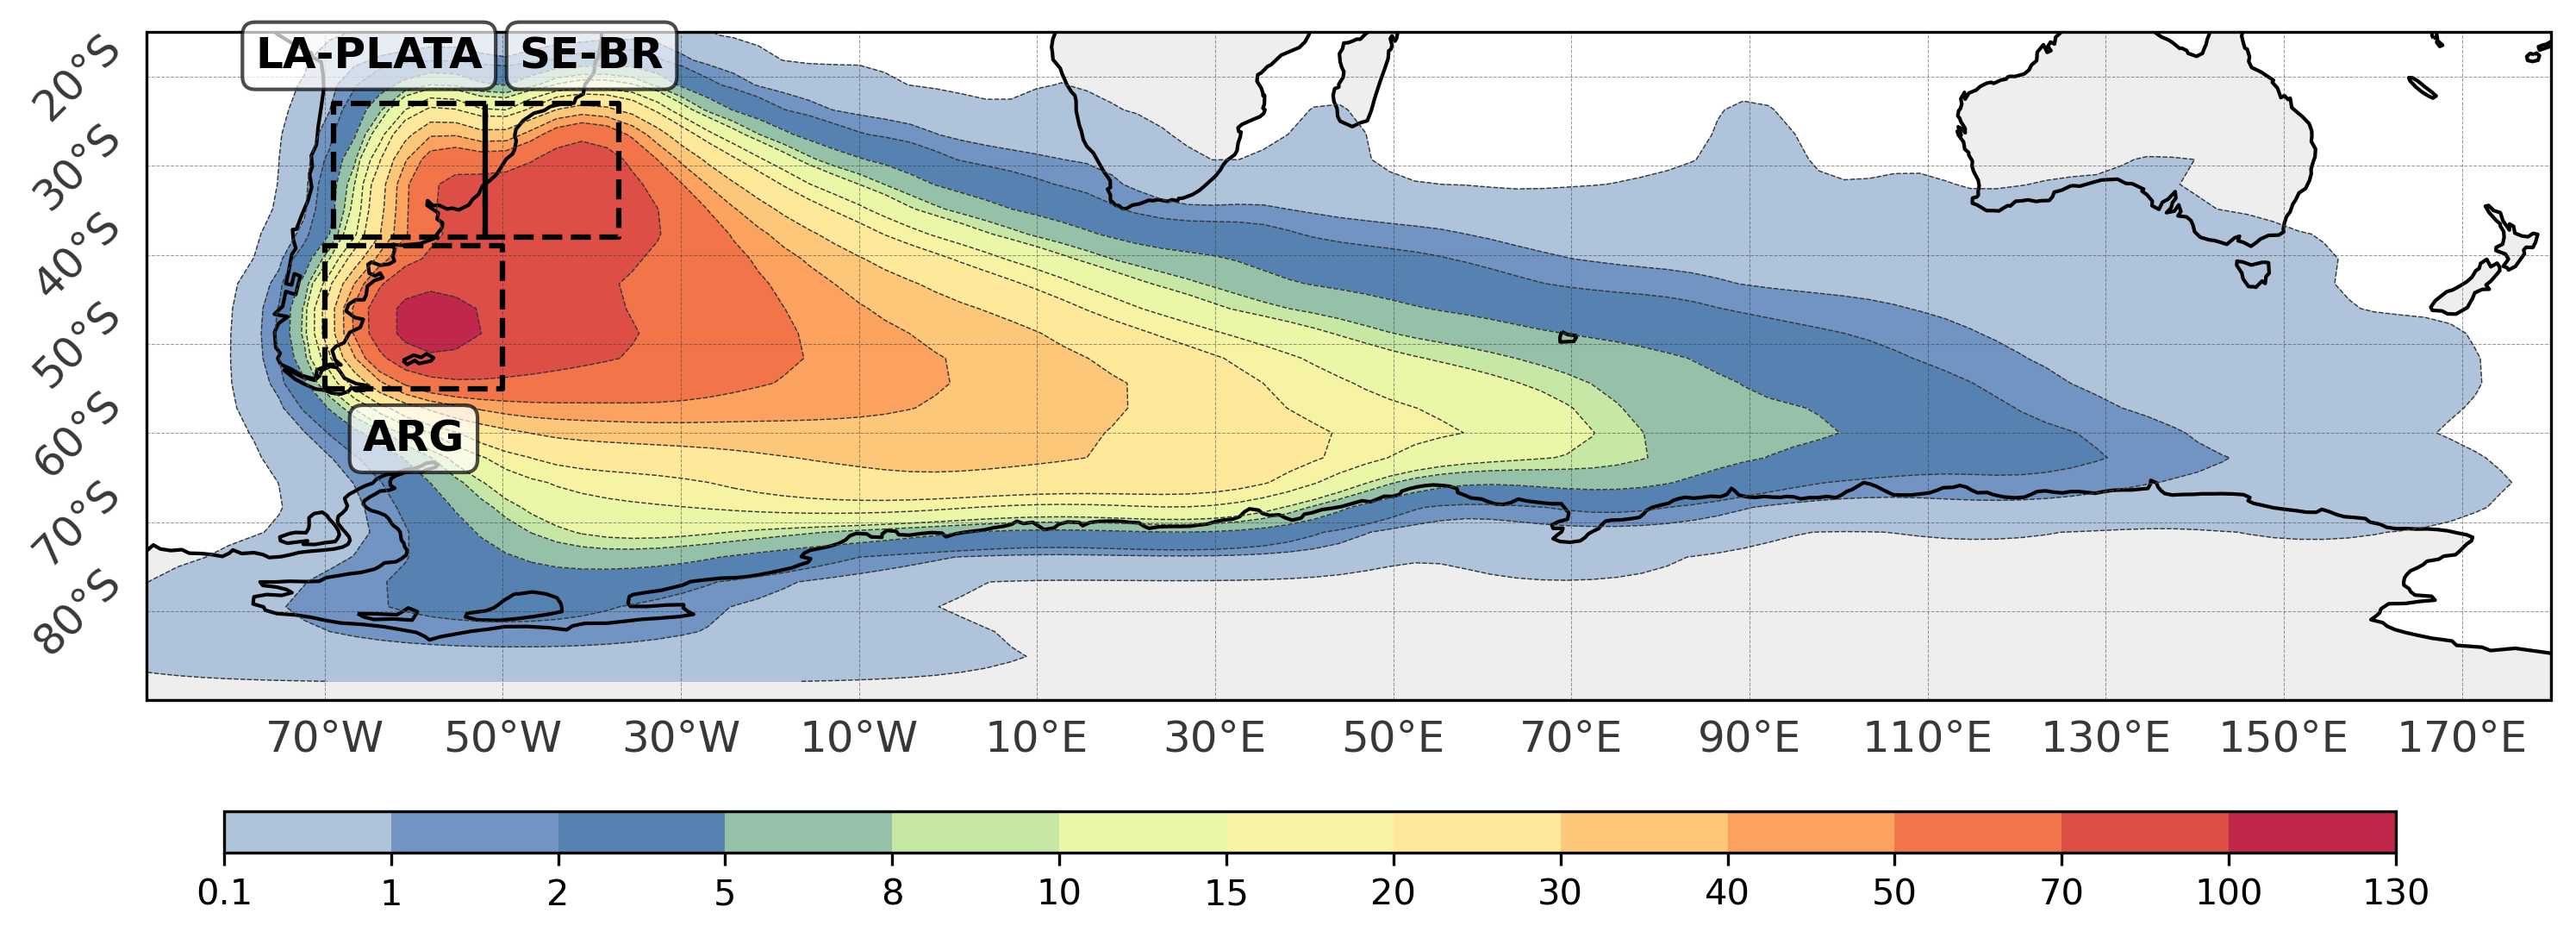
\includegraphics[width=\textwidth]{combined_density_map_all_phases_regions_with_regions.png}
    \caption{Cyclone track density for all systems analyzed in this study, highlighting the cyclogenesis regions near the South American coast (ARG, LA-PLATA, and SE-BR). The track density unit is cyclone per $10^{6}$ $km^{2}$ per month.}
    \label{fig:combined_density_map_all_phases_regions_with_regions}
\end{figure}


\subsection{Lorenz Energy Cycle Computation}

For computing the LEC, we used the the open-source Python application LorenzCycleToolKit \citep{de2024lorenzcycletoolkit}. The energy budget equations for the zonal and eddy forms of APE and kinetic energy are then expressed as:

\begin{flalign}
\frac{\partial A_Z}{\partial t} &= BA_Z - C_Z - C_A + G_Z \\
\frac{\partial A_E}{\partial t} &= BA_E - C_E + C_A + G_E \\
\frac{\partial K_Z}{\partial t} &= BK_Z + C_Z - C_K + B\Phi_Z - D_Z \\
\frac{\partial K_E}{\partial t} &= BK_E + C_E + C_K + B\Phi_E - D_E 
\end{flalign}

In these equations, APE is divided into zonal (\(A_Z\)) and eddy (\(A_E\)) components, as is kinetic energy (\(K_Z\) and \(K_E\), respectively). \(C_A\) represents the conversion between \(A_Z\) and \(A_E\), \(C_E\) denotes the conversion from \(A_E\) to \(K_E\), \(C_K\) signifies the transformation from \(K_E\) to \(K_Z\), and \(C_Z\) describes the conversion from \(A_Z\) to \(K_Z\). Generation of APE and dissipation of kinetic energy are indicated by \(G\) and \(D\), with \(G_Z\) and \(G_E\) marking the generation of \(A_Z\) and \(A_E\), and \(D_Z\) and \(D_E\) representing the dissipation of \(K_Z\) and \(K_E\), respectively. \(BA_Z\), \(BA_E\), \(BK_Z\), and \(BK_E\) represent, respectively, the flows of zonal and eddy APE and K across the boundaries. The terms \(B\Phi_Z\) and \(B\Phi_E\) are represented together with the terms \(C_Z\) and \(C_E\), respectively, because both arise from the same process of deriving the balances of \(K_Z\) and \(K_E\). \citet{muench1965dynamics} recognizes the difficulty in interpreting the terms \(B\Phi_Z\) and \(B\Phi_E\), indicating that they are related to the flow of kinetic energy towards lower altitudes, representing the emergence of kinetic energy at the boundaries of the computational domain. For the full mathematical formulations for these processes we refer to the original \citet{muench1965dynamics} and \citet{brennan1980zonal} formulations. 


Following the methodologies of \citet{brennan1980zonal,michaelides1987limited,veiga2008analysis,pezza2010environmental,dias2011energy}, the program was set to compute the generation, dissipation and boundary pressure work terms (\(B\Phi_Z\) and \(B\Phi_E\)) as residuals, defined as:

\begin{flalign}\label{residuo_Michaelides}
RK_Z &= B\Phi_Z - D_Z + \epsilon_{KZ} \\
RK_E &= B\Phi_E - D_E + \epsilon_{KE} \\
RG_Z &= G_Z + \epsilon_{GZ} \\
RG_E &= G_E + \epsilon_{GE}
\end{flalign}

Where $\epsilon$ account for numerical errors in the computation procedures. The set of budget equations becomes, then: 

\begin{flalign}\label{balanco_Brennan}
\frac{\partial A_Z}{\partial t} &= -C_A - C_Z + RG_Z + BA_Z \\
\frac{\partial A_E}{\partial t} &= C_A - C_E + RG_E + BA_E  \\
\frac{\partial K_Z}{\partial t} &= C_K + C_Z + BK_Z + RK_Z \\
\frac{\partial K_E}{\partial t} &= - C_K + C_E + BK_E  + RK_E 
\end{flalign}

A complete deciption of the LEC, with arrows indicating positive energy fluxes, is presented in Figure \ref{fig:LEC_Michaelides}.


\begin{figure}[htbp]
    \centering
    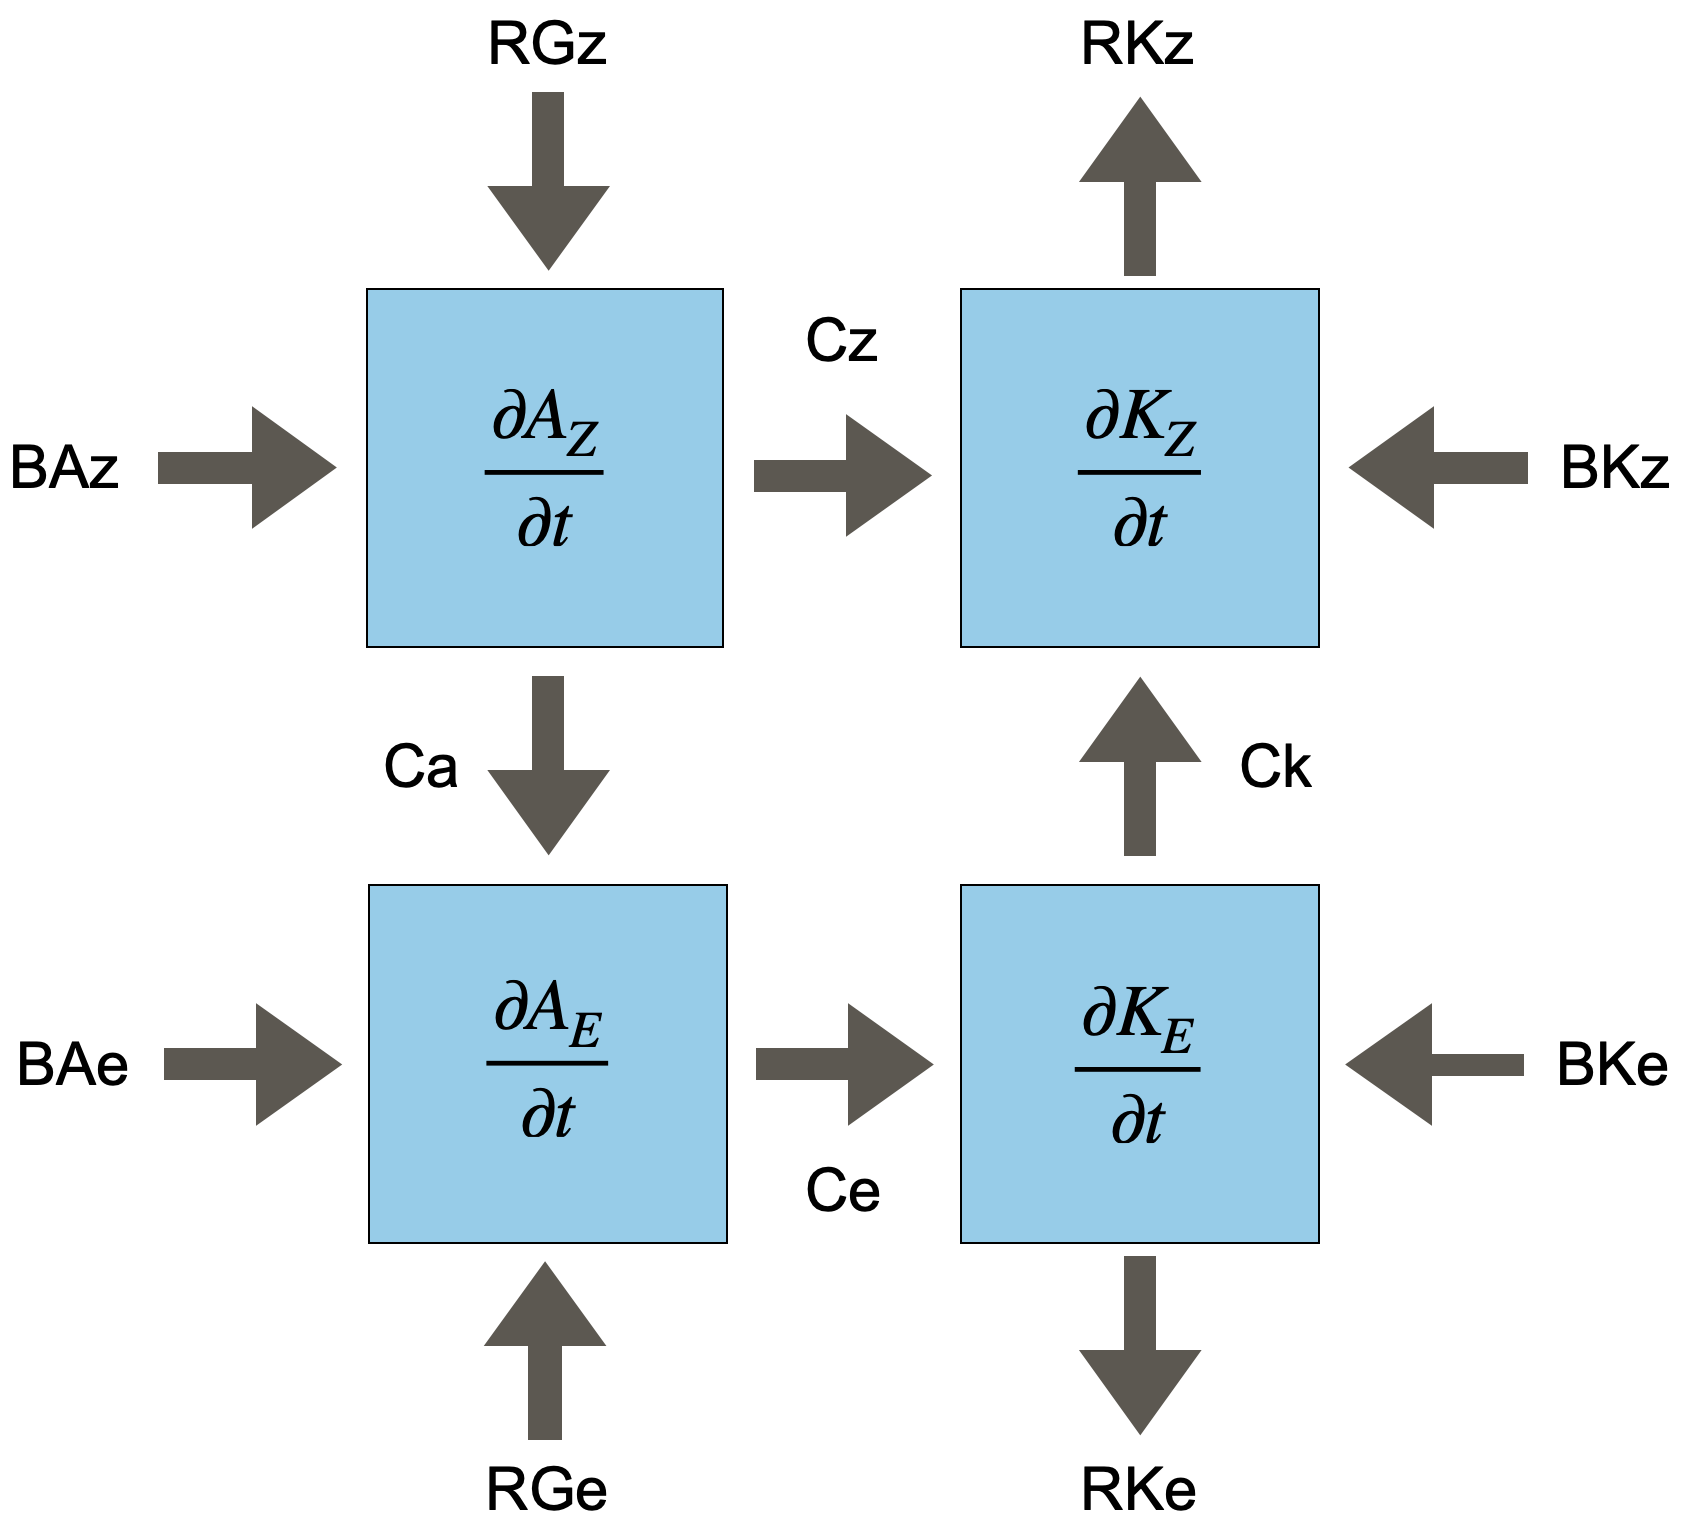
\includegraphics[width=\textwidth]{LEC_Michaelides.png}
    \caption{Representation of the Lorenz Energy Cycle (LEC), with arrows denoting positive energy fluxes.}
    \label{fig:LEC_Michaelides}
\end{figure}

Here, we used a Semi-Lagrangian framework \citep{michaelides1999quasi}, aiming to minimize interactions with other non-related circulations while capturing the main structure of the cyclone. A $15^\circ \times 15^\circ$ computational domain centered at the cyclone's central position, obtained from the TRACK database, was created for each time step. Given the impracticality of manually selecting an appropriate domain size for each cyclone in the dataset, a fixed size was employed. The choice of a $15^\circ \times 15^\circ$ computational domain is justified as it is large enough to capture the effective radius of most cyclonic systems \citep{rudeva2007climatology}. The effective cyclone radius is defined as a measure of cyclone size, determined by establishing a coordinate system centered on the cyclone and measuring the distance at which the radial pressure gradient first falls to zero. This domain size also is large enough for accommodating the cyclone's synoptic structure \citep[e.g.][]{gramcianinov2019properties}.


\subsection{Analysis Methods}

A key challenge in computing the LEC for large datasets lies in the variable life durations of cyclones. Averaging energy values across an entire life cycle can obscure distinct dynamical processes tied to different stages of cyclone development, while technical limitations exist in dissecting the life cycle into distinct periods. For example, \citet{black2013universal} averaged cyclone energetics over periods of 48 hours before explosive cyclogenesis, during explosive deepening, and for 24 and 72 hours after it. However, cyclone life cycles can range from less than 24 hours to over 10 days \citep{trigo2006climatology,reboita2010south,gramcianinov2019properties}, presenting significant physical limitations to such approaches.

To address these issues, we employed Cyclophaser, an open-source Python package designed to detect cyclone life cycle phases using time series of relative vorticity at the system's central position and its first derivative \citep{deSouza2024CycloPhaser}. Cyclophaser applies a series of preprocessing steps, including Lanczos \citep{duchon1979lanczos} and Savitzky-Golay \citep{savitzky1964smoothing} filtering, to smooth the data and remove noise from mesoscale influences on the relative vorticity series, such as sea-breeze phenomena, wind interaction with coastal topography, and sea surface structures \citep[e.g.][]{steele2015modelling,da2017shallow,acevedo2010atmospheric}. The program identifies intensification, decay, mature, and residual phases based on peaks and valleys in the vorticity and its derivative, applying threshold criteria for phase duration and significance.

In this study, we utilized the same life cycle detection approach as \citet{CycloPhaser2024}. For a detailed description of the procedure, spatial distribution of cyclone life cycle phases in the South Atlantic, and statistics such as duration, displacement, speed, and intensity for each phase, see \citet{couto2024new}. After computing the LEC for each system, Cyclophaser was used to define the life cycle phases for all analyzed systems, followed by the computation of mean LEC values for each phase. This approach allows us to investigate the dynamical mechanisms specific to each development phase. For instance, it is expected that distinct energy fluxes will dominate during the intensification and decay phases, especially in the atmospheric region near the cyclone center.

To understand the dominant LEC variability patterns within the TRACK dataset, we performed an Empirical Orthogonal Function (EOF) analysis \citep{fukuoka1951study,lorenz1956empirical} using the Python open-source library pyEOF \citep{zheng_2021}. This analysis reduces the dimensionality of the dataset, retaining the most significant variability, and is particularly useful for uncovering underlying structures and patterns in complex environmental data. Typically, each EOF represents a spatial pattern, while the associated time series, or Principal Component (PC), describes the temporal evolution of that pattern. However, in this study, instead of representing a spatial pattern, each EOF reflects a mode of variability in the LEC, while the PCs represent the evolution across individual cyclones, which are not displayed as they do not represent any meaningful physical feature. In this study, the EOF analysis was performed separately for data corresponding to each life cycle phase, enabling a more detailed examination of variability throughout the cyclone's development, but also for the cyclones complete energy cycle.

To associate cyclones with predominant EOFs, we first project each cyclone's energetics onto the PCs obtained from an EOF analysis. This allows us to represent each system in terms of its contribution to the dominant modes of variability. Then we classify cyclones into EOF(+) and EOF(-) groups, from identify systems where at least one PC reaches extreme values. Specifically, EOF(+) are cyclones for which at least one PC exceeds the 90th percentile (q90), indicating strong positive projection onto a specific mode. Meanwhile, EOF(-) are  cyclones for which at least one PC is below the 10th percentile (q10), indicating strong negative projection onto a specific mode. For each cyclone meeting these criteria, we determine its predominant EOF as the one corresponding to the PC with the highest absolute value. This ensures that each system is classified based on the mode that most strongly characterizes its structure and dynamics.

For determining the LEC patterns of the most intense systems, we first selected only the cyclones in which the maximum central vorticity at 850 hPa exceeded the 99th percentile of the dataset. Subsequently, we applied the K-Means algorithm to identify groups within these cyclones' PCs. K-Means is an unsupervised learning algorithm that partitions data into \( K \) clusters by minimizing intra-cluster variance while maximizing separation between groups based on sample similarity \citep{macqueen1967,hartiganwong1979}. The optimal number of clusters was determined using the Elbow Method, which identifies the most suitable number of clusters by plotting the within-cluster sum of squares for different values of \( K \) and locating the "elbow point," where the rate of decrease slows, indicating a balance between model complexity and performance. For this analysis, we employed the K-Means implementation from the \texttt{scikit-learn} Python package \citep{hao2019machine} and used the \texttt{yellowbrick} package for the Elbow Method \citep{bengfort2019yellowbrick}.




\section{Results}\label{sec:results}

\subsection{Climatological Features}\label{sec:climatology}

The exploratory statistical metrics for all LEC terms can be found in Table \ref{tab:lec_stats}, while their probability density functions (PDFs) are shown in Figure \ref{fig:combined_ridge}. Notably, all terms related to the zonal jets ($K_Z$, $BK_Z$, and \(\frac{\partial K_Z}{\partial t}\)) frequently exhibit statistical metrics one order of magnitude higher than their eddy counterparts within the same group ($K_E$, $BK_E$, and \(\frac{\partial K_E}{\partial t}\)), indicating significantly greater energy amount concentrated on the jet streams. Although the energy budgets were computed with the generation and dissipation terms calculated as residuals, the generation terms can be directly computed using ERA5 data. Therefore, their probability density functions (PDFs) are also shown for a more physically based analysis (Figure \ref{fig:combined_ridge}e). Furthermore, the comparison between the directly computed generation values and those estimated by residual computation provides a useful metric for evaluating the accumulation of errors in LEC computation procedure. The dissipation terms were not directly computed in the present study.

All the energy terms (\textit{Kz}, \textit{Az}, \textit{Ae}, and \textit{Ke}, Figure \ref{fig:combined_ridge}a) exhibit right-skewed distributions. Among these, $A_Z$ shows the largest variability, as reflected in its long-tail distribution, standard deviation (std), interquartile range (IQR), and range, compared to $A_E$ and $K_E$, peaking at approximately $4 \times 10^5 \, J \, m^{-2}$. Conversely, $A_E$ presents the lowest variability, peaking near $1 \times 10^5 \, J \, m^{-2}$, closer to its mean value. The kinetic energy terms, $K_Z$ and $K_E$, display similar distributions, with $K_Z$ peaking near $20 \times 10^5 \, J \, m^{-2}$ and $K_E$ peaking near $2 \times 10^5 \, J \, m^{-2}$.

\begin{table}[!htbp]
\centering
\caption[Summary Statistics of Lorenz Energetics Components]{Summary Statistics of Lorenz Energetics Components: mean, median, standard deviation (std), 25th percentile (Q25), 75th percentile (Q75), interquantile range (IQR), and range. The IQR measures the range within which the central 50\% of the values fall, while the range is computed as the difference between the maximum and minimum values. The units for the energy terms ($A_Z$, $A_E$, $K_Z$, and $K_E$) are $10^5 \, J \, m^{-2}$ and $W \, m^{-2}$ for the remaining terms.}
\label{tab:lec_stats}
\begin{tabular}{lrrrrrrr}
\toprule
Term & Mean & Median & Std Dev & Q25 & Q75 & IQR & Range \\
\midrule
Az & 5.55 & 4.68 & 3.71 & 2.77 & 7.49 & 4.72 & 36.46 \\
Ae & 1.62 & 1.24 & 1.20 & 0.77 & 2.09 & 1.32 & 11.07 \\
Kz & 28.55 & 26.19 & 15.10 & 17.34 & 37.12 & 19.78 & 114.55 \\
Ke & 3.70 & 2.95 & 2.62 & 1.92 & 4.63 & 2.71 & 24.81 \\
Cz & 0.52 & 0.38 & 4.85 & -1.96 & 2.92 & 4.89 & 86.70 \\
Ca & 0.93 & 0.46 & 1.57 & 0.02 & 1.44 & 1.41 & 19.78 \\
Ck & -3.56 & -1.63 & 9.51 & -5.77 & 0.47 & 6.24 & 206.43 \\
Ce & 3.84 & 2.47 & 4.92 & 0.63 & 5.84 & 5.21 & 54.74 \\
BAz & 3.54 & 2.03 & 7.67 & -0.67 & 6.67 & 7.34 & 175.05 \\
BAe & 0.58 & 0.16 & 4.40 & -1.13 & 2.02 & 3.15 & 75.72 \\
BKz & -7.93 & -5.53 & 31.75 & -23.75 & 7.83 & 31.58 & 445.63 \\
BKe & 0.47 & 0.08 & 8.59 & -2.73 & 3.22 & 5.95 & 146.87 \\
$B\Phi Z$ & 63.87 & 49.25 & 128.05 & -9.12 & 132.35 & 141.47 & 1419.08 \\
$B\Phi E$ & 39.66 & 31.19 & 126.50 & -28.84 & 109.47 & 138.32 & 1353.99 \\
Gz & -0.31 & -0.17 & 2.66 & -1.39 & 0.81 & 2.21 & 68.74 \\
Ge & 1.17 & 0.56 & 3.14 & -0.26 & 2.21 & 2.46 & 58.39 \\
$\frac{\partial A_z}{\partial t}$ & -0.07 & -0.14 & 4.46 & -2.04 & 1.68 & 3.71 & 106.39 \\
$\frac{\partial A_e}{\partial t}$ & -0.23 & -0.10 & 1.92 & -0.85 & 0.51 & 1.35 & 48.19 \\
$\frac{\partial K_z}{\partial t}$ & 1.59 & 0.75 & 13.38 & -5.33 & 8.15 & 13.48 & 251.24 \\
$\frac{\partial K_e}{\partial t}$ & 0.28 & 0.12 & 3.18 & -1.13 & 1.58 & 2.71 & 61.50 \\
RGz & -2.17 & -1.00 & 7.60 & -5.22 & 1.56 & 6.78 & 220.06 \\
RKz & 12.56 & 8.69 & 40.49 & -8.68 & 32.71 & 41.39 & 561.24 \\
RGe & 2.10 & 1.20 & 5.15 & -0.40 & 4.21 & 4.61 & 97.25 \\
RKe & -7.59 & -4.63 & 10.62 & -11.48 & -1.04 & 10.43 & 138.42 \\
\bottomrule
\end{tabular}
\end{table}

For the conversion terms, $C_Z$, $C_K$, and $C_E$ exhibit high variability, in contrast to $C_A$. The former terms display long-tail distributions, peaking near zero, $-1$, and $2 \, W \, m^{-2}$, respectively, while $C_A$ presents a narrow distribution with a sharp peak near its mean value, close to zero (Figure \ref{fig:combined_ridge}b). The $C_Z$ probability density function (PDF), along with the mean and quantile values, and its mean value being close to the median, indicate an overall tendency for both $A_Z \rightarrow K_Z$ and $K_Z \rightarrow A_Z$ conversions. However, the positive mean and median values suggest a predominant $A_Z \rightarrow K_Z$ pathway. For $C_A$ and $C_E$, the metrics presented in Table \ref{tab:lec_stats} indicate a consistent tendency for positive conversions, corresponding to $A_Z \rightarrow A_E \rightarrow K_E$ (baroclinic chain), but with more modest $A_Z \rightarrow A_E$ conversions than $A_E \rightarrow K_E$. In the case of the $C_K$ term (barotropic conversion term), the metrics indicate a predominant negative conversion, i.e., $K_Z \rightarrow K_E$, although the positive Q75 value suggests the occurrence of events where $K_E \rightarrow K_Z$ conversions also take place.

\begin{figure}[htbp]
    \centering
    
\includegraphics[width=\textwidth]{combined_ridge.png}
    \caption{Probability density function (PDF) plots for distinct Lorenz Energetics terms: (A) energy, (B) conversion, (C) boundary, (D) pressure work, (E) generation and residual, and (F) budget terms. The x-axis represents the energy values, while the y-axis represents density counts. The units for the energy terms ($A_Z$, $A_E$, $K_Z$, and $K_E$) are in $10^5 \, J \, m^{-2}$, and in $W \, m^{-2}$ for the remaining terms. Terms related to $K_Z$ are divided by 10 (*) to account for their order of magnitude difference, which would otherwise distort the visualization.}
    \label{fig:combined_ridge}
\end{figure}

For the boundary terms, $BA_E$ and $BK_Z$ exhibit similar distributions, as do $BA_Z$ and $BK_E$ (Figure \ref{fig:combined_ridge}c). The terms $BA_E$ and $BK_E$ display narrow distributions, peaking near zero, whereas $BA_Z$ and $BK_Z$ show nearly symmetrical long-tail distributions. Although for all four terms, both positive (influx) and negative (outflux) energy fluxes occur, as indicated by their negative Q25 and positive Q75 values, the peak near zero for $BA_E$ and $BK_Z$ suggests that boundary energy fluxes are typically low in most cases. In contrast, for $BA_Z$, the peak near $2 \, W \, m^{-2}$ indicates an overall tendency for energy influx, while for $BK_E$, the peak near $-2 \, W \, m^{-2}$ points to a predominant tendency for energy outflux. Meanwhile, the boundary pressure work terms ($B\Phi Z$ and $B\Phi E$) exhibit significantly higher values compared to the other boundary terms, with both presenting nearly symmetric distributions (Figure \ref{fig:combined_ridge}d). These terms show tail distributions exceeding $\pm 200 \, W \, m^{-2}$, indicating substantial variability. These terms will be discussed in detail later.

Overall, both generation terms ($G_Z$ and $G_E$) present nearly symmetrical distributions centered near zero (Figure \ref{fig:combined_ridge}e), suggesting that in most cases, either the zonally averaged diabatic heating ($G_Z$) and the zonal deviations ($G_E$) are low, or the atmospheric stability is high. However, there are instances where this behavior is amplified ($G < 0$) or reversed ($G > 0$). In contrast, the generation residual terms ($RG_Z$ and $RG_E$) display distinct characteristics. The $RG_Z$ term is left-skewed, with a long-tail distribution and higher variability compared to $G_Z$, as indicated by its lower Q25 and higher Q75 and IQR values (Table \ref{tab:lec_stats}). Additionally, $RG_Z$ exhibits more negative mean and median values than $G_Z$, suggesting a bias toward processes such as diabatic cooling at lower latitudes and/or heat distribution mechanisms that reduce zonal temperature gradients, such as cyclonic activity. On the other hand, $RG_E$ is more symmetrical than $RG_Z$, though it still shows higher variability compared to $G_E$, as evidenced by its lower Q25 and higher Q75 and IQR values. Moreover, $RG_E$ exhibits higher mean and median values than $G_E$, indicating a bias toward overestimating the eddy effects on latent heat release and meridional temperature gradients. Therefore, the residuals suggest that the computed LEC increases the contribution of eddy motions to the atmospheric energy cycle through enhanced meridional heat transport, reducing zonal temperature gradients and enhancing convective activity within cyclone frontal structures.

Similar to the generation residual terms, each dissipation residual term displays distinct distributions (Figure \ref{fig:combined_ridge}e). The PDF for $RK_Z$ mirrors that of $RG_E$, showing modest variability. Its negative Q25 values indicate instances of net dissipation of $K_Z$. However, the high positive mean, median, Q75, and IQR values suggest that in most cases, there is a net increase of $K_Z$ related to this term, possibly due to the high $B\Phi Z$ value. In contrast, $RK_E$ shows high variability with a left-skewed, long-tail distribution. Both its Q25 and Q75 are negative, indicating that dissipation of $K_E$ frequently occurs.

\subsection{Mean Energy Values Across Life Cycle Phases}\label{sec:mean}

The use of the CycloPhaser program allowed for the application of an objective criterion to dissect the cyclones into distinct life cycle phases, enabling an investigation of their energy cycles across these phases (Figure \ref{fig:panel_lec_mean_phases}). Our analysis revealed that the mean energy flow directions rarely change across phases, although the magnitude of each term varies. However, the high standard deviation values indicate that energy fluxes frequently deviate from their mean direction.

The $A_Z$ budget term exhibits mean positive values during the incipient phase, which turn negative during the intensification and mature phases, becoming positive again during the decay phase. The mean $K_Z$ budget values are positive throughout all phases except during the mature phase. In contrast, the $A_E$ budget remains negative across the entire life cycle, while the $K_E$ budget is positive during the incipient and intensification phases but turns negative during the mature and decay phases.

Across the different cyclone phases, the mean behavior suggests that both baroclinic and barotropic conversions remain active, continuously providing energy to the eddies. There is a marked enhancement of baroclinic conversions from the incipient to intensification phase, which then decrease in magnitude during the mature and decay phases. Conversely, barotropic conversion peaks during the mature phase, surprisingly with a higher magnitude than the $A_E \rightarrow K_E$ conversion. The behavior of the baroclinic chain is mirrored by the $G_E$ term, which begins with negative values and, during the intensification phase, reaches a higher magnitude than the $C_A$ term. The $G_Z$ term remains negative throughout the entire life cycle, with progressively decreasing values.

Throughout the life cycle, the mean values indicate imports of $A_Z$, which decrease in the mature phase but rise again during the decay phase. The mean $BA_E$ values exhibit a bimodal behavior, being positive during the incipient and intensification phases but turning negative during the mature and decay phases, though with negligible mean values in the latter.

Across all phases, the $RK_Z$ term stands out with the highest mean values, also displaying the greatest variability, as indicated by the high standard deviation values. This could be influenced by the $B\Phi Z$ term, as mentioned in the previous section. The $BK_Z$ term also presents high mean values and variability across all phases, suggesting a compensatory effect for the excess energy from the $RK_Z$ term. Lastly, the mean $RK_E$ values are negative across all phases, peaking during the mature phase, indicating significant dissipation in this phase and presenting similar values during the incipient and decay phases.


\begin{figure}[!htbp]
\centering

\includegraphics[width=\textwidth]{panel_lec_mean_phases.pdf}
\caption{Mean values and standard deviation of the limited-area Lorenz Energy Cycle (LEC) terms for each life cycle phase : incipient (A), intensification (B), mature (C), and decay (D). Each box represents an energy component ($\, J \, m^{-2}$), with arrows showing the direction of energy flow ($\, W \, m^{-2}$). The numbers adjacent to the arrows indicate the magnitude and direction of the energy flux, with green indicating positive values and red indicating negative values}
\label{fig:panel_lec_mean_phases}
\end{figure}

\subsection{Empirical Orthogonal Function Analysis}\label{sec:eof}

The variance explained by the first eight Empirical Orthogonal Functions (EOFs) highlights the dominant modes of variability in the dataset. The first EOF accounts for 28.3\% of the total variance, capturing the primary mode of variability, while the second and third EOFs each explain approximately 11.0\% and 10.9\%, respectively. Subsequent EOFs contribute progressively smaller amounts, with the fourth, fifth, sixth, seventh, and eighth EOFs explaining 8.2\%, 7.4\%, 5.9\%, 5.2\%, and 4.4\%, respectively. The cumulative variance explained by the first eight EOFs provides insight into the primary modes of variability in the dataset, with diminishing returns beyond the initial EOFs. Typically, the principal components (PCs, not shown) represent the signal magnitude associated with each EOF. However, in this context, they primarily reflect the signal magnitude across the distinct cyclones and, therefore, do not represent any specific temporal physical feature. In this study, emphasis is placed on the first four EOFs. Additionally, while the interpretation of the EOF signal can consider both positive and negative contributions, for simplicity, we focus exclusively on the positive contributions.

Figure \ref{fig:eof1_phases} illustrates the Lorenz Energy Cycle (LEC) terms associated with EOF 1. Across all life cycle phases, there is a consistent enhancement of moist baroclinic conversions, characterized by the positive values of the $A_Z \rightarrow A_E \rightarrow K_E$ conversions, in conjunction with an enhancement of the $G_E$ term. Furthermore, there is an increase in the $K_Z \rightarrow K_E$ conversion ($C_K$ becomes more negative), particularly during the mature and decay phases. These variations largely reinforce the mean behavior observed across the cyclone's life cycle. In addition, $A_Z$ imports are enhanced, while a negative tendency is observed in its budget and generation terms. Conversely, the $K_Z$ boundary, budget, and residual terms show a positive tendency. Lastly, the $C_Z$ term presents a weak positive signal during the incipient and decay phases, and a negative tendency during the intensification and mature phases.

\begin{figure}[!htbp]
\centering
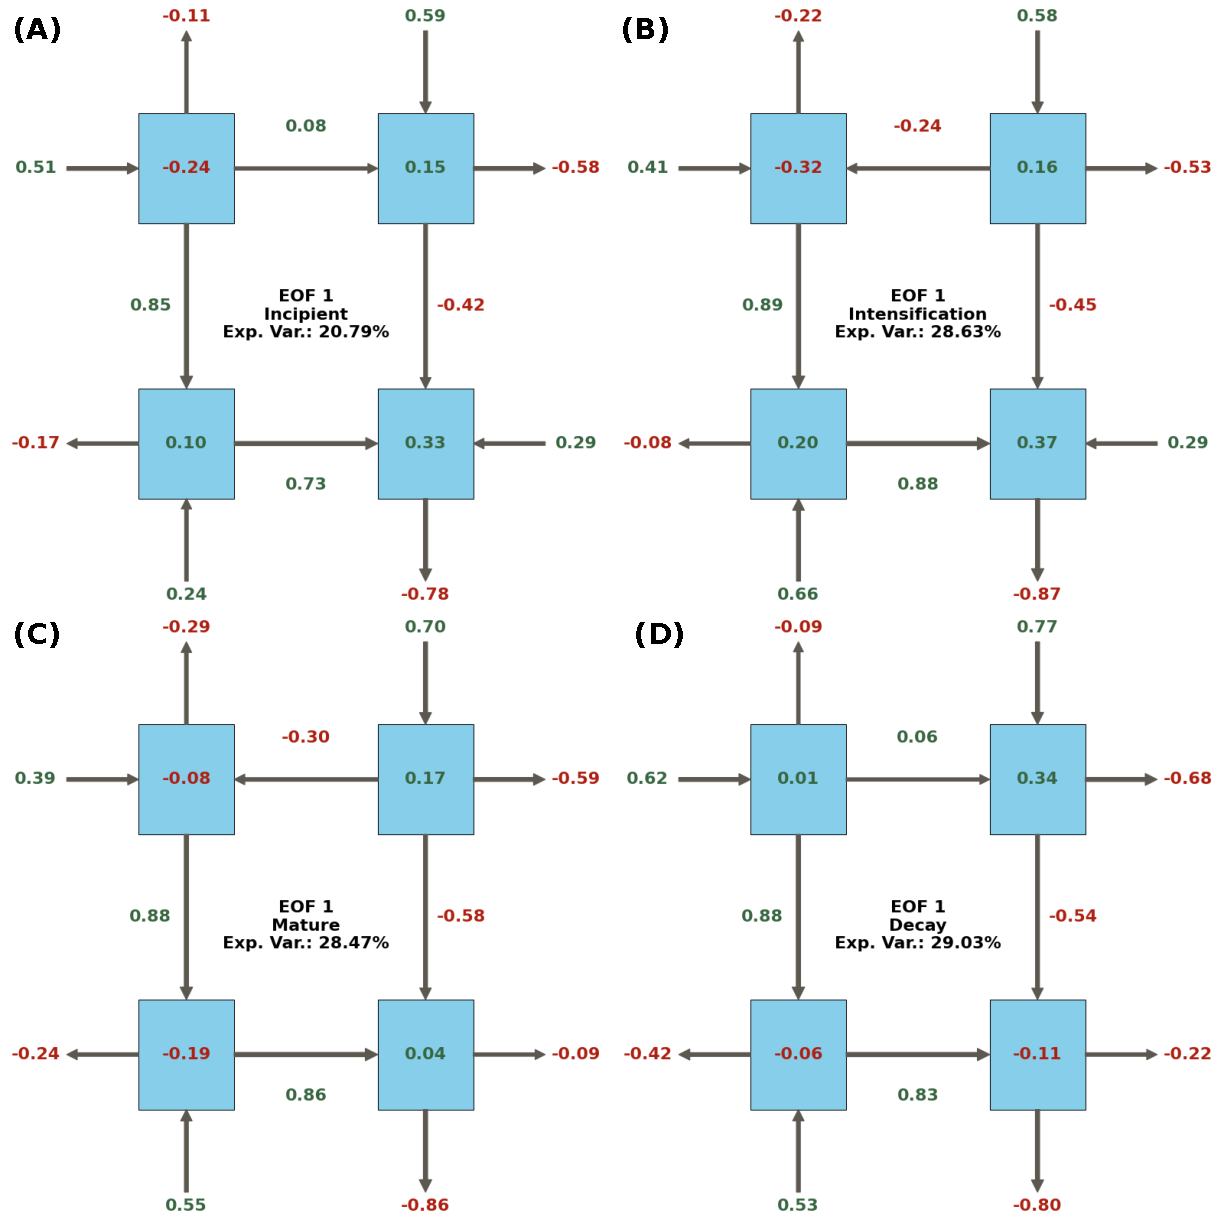
\includegraphics[width=\textwidth]{eof1_phases.pdf}
\caption{Lorenz Energy Cycle (LEC) terms for the first Empirical Orthogonal Function (EOF 1) across different life cycle phases: (A) incipient, (B) intensification, (C) mature, and (D) decay.}
\label{fig:eof1_phases}
\end{figure}

During the incipient (Figure \ref{fig:eof2_phases}A) and intensification phases (Figure \ref{fig:eof2_phases}B), EOF 2 displays an overall weakening of the $C_A$ term, in contrast to EOF 1. Additionally, there is a reduction in barotropic conversions, indicating a $K_E \rightarrow K_Z$ tendency, alongside a weakening of $K_E$ imports. This reduction is compensated by an enhancement in $A_E$ imports, which appears to be the primary mechanism driving the increase in the $C_E$ term. In the mature phase (Figure \ref{fig:eof2_phases}C), the signal for $A_E$ imports reverses in sign, and an enhancement of the moist baroclinic chain occurs, accompanied by a slight increase in $K_Z \rightarrow K_E$ conversions and a more pronounced increase in $K_E$ imports. During the decay phase (Figure \ref{fig:eof2_phases}D), both the moist baroclinic chain and $K_Z$ imports show a negative tendency. However, the enhanced barotropic conversions, coupled with a weakening of dissipation (positive tendency for $RK_E$), result in a slight yet positive tendency in $K_E$, suggesting a slower dissipation process.

\begin{figure}[!htbp]
\centering
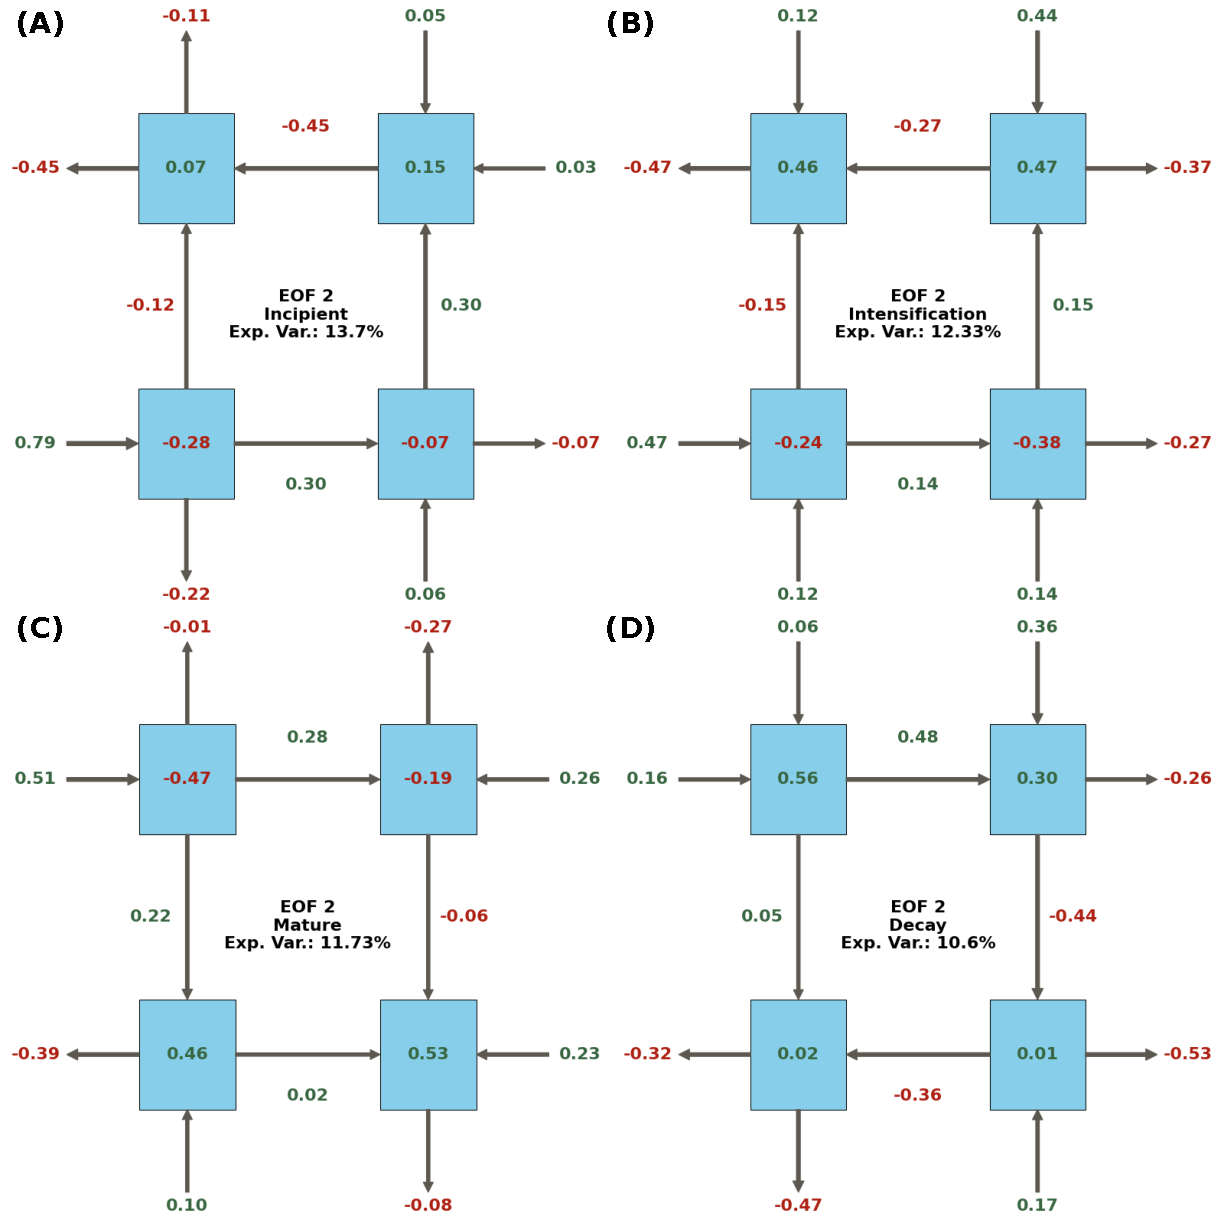
\includegraphics[width=\textwidth]{eof2_phases.pdf}
\caption{Lorenz Energy Cycle (LEC) terms for the second Empirical Orthogonal Function (EOF 2) across different life cycle phases: (A) incipient, (B) intensification, (C) mature, and (D) decay.}
\label{fig:eof2_phases}
\end{figure}

For EOF 3 (Figure \ref{fig:eof3_phases}), the role of the moist baroclinic chain diminishes in eddy development. This is evident from the weakening of the $C_E$ and $G_E$ terms across the incipient (Figure \ref{fig:eof3_phases}A), intensification (Figure \ref{fig:eof3_phases}B), and mature (Figure \ref{fig:eof3_phases}C) phases, although the $C_A$ term shows a slight enhancement during these phases. In the incipient phase, the primary mechanism driving eddy growth is $K_Z$ imports. However, during the intensification and mature phases, the dominant source of energy shifts to barotropic conversions.During the decay phase (Figure \ref{fig:eof3_phases}D), the marginal enhancement of the $C_E$ term is driven by a slight increase in the $G_E$ term and, more importantly, by an enhancement of $A_E$ imports. Although this works in conjunction with increased $K_E$ imports, the simultaneous enhancement of $K_E \rightarrow K_Z$ conversions leads to the dissipation of eddies.


\begin{figure}[!htbp]
\centering
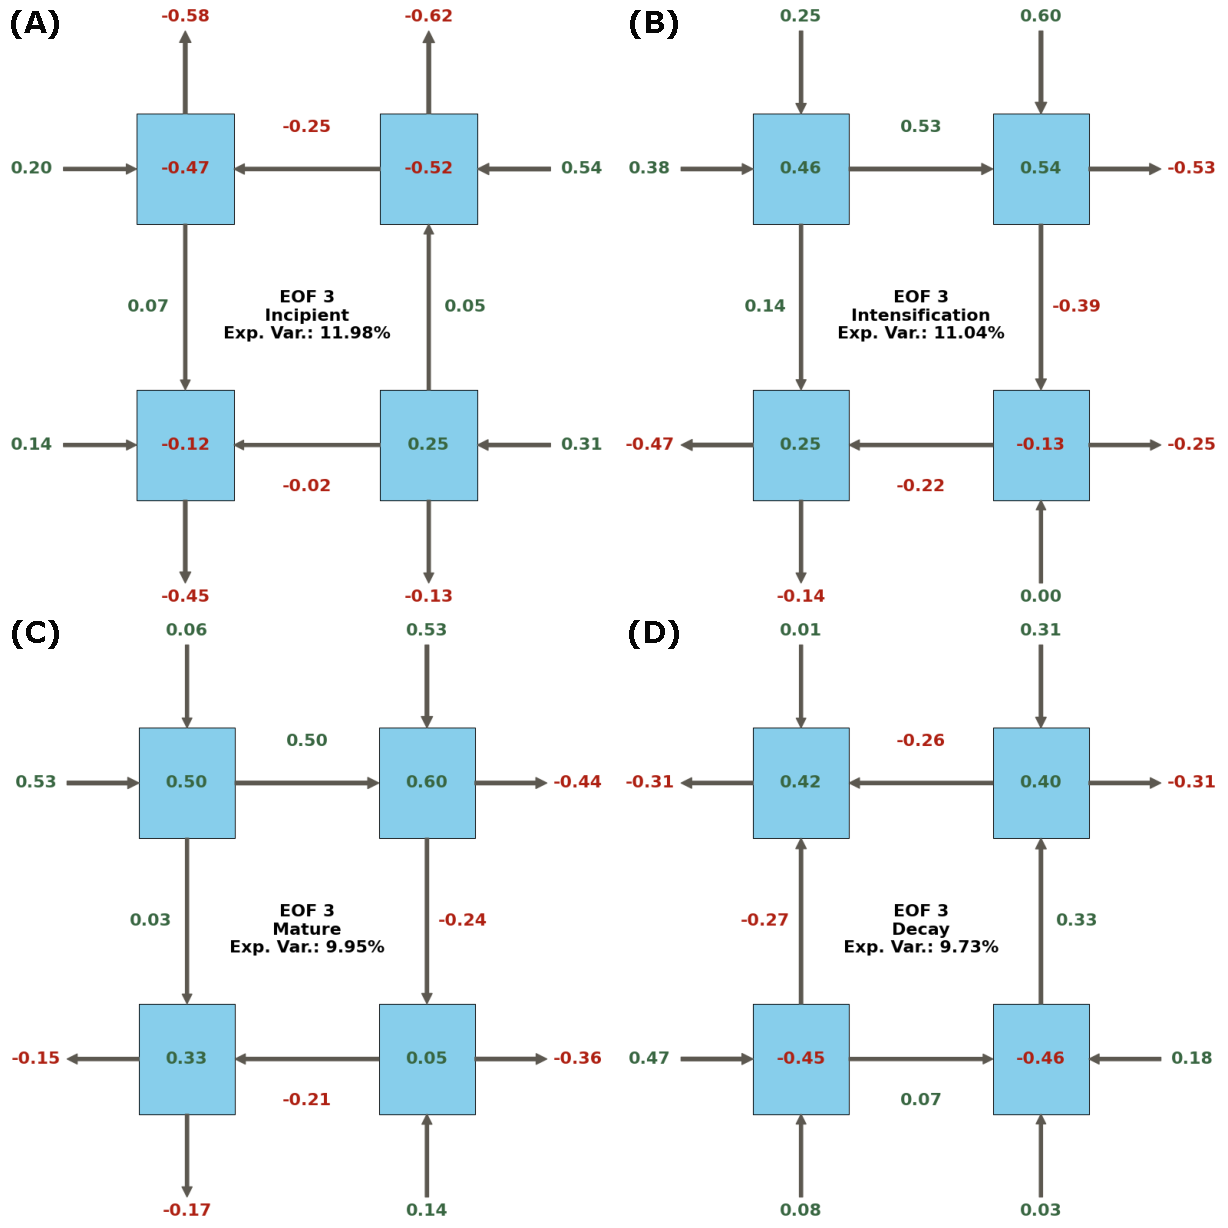
\includegraphics[width=\textwidth]{eof3_phases.pdf}
\caption{Lorenz Energy Cycle (LEC) terms for the third Empirical Orthogonal Function (EOF 3) across different life cycle phases: (A) incipient, (B) intensification, (C) mature, and (D) decay.}
\label{fig:eof3_phases}
\end{figure}

During the incipient phase (Figure \ref{fig:eof4_phases}A) of EOF 4, the moist baroclinic chain weakens, as do the $K_E$ imports, while the barotropic conversions are enhanced. As the system progresses to the intensification phase (Figure \ref{fig:eof4_phases}B), the barotropic conversion signal becomes neutral, and the weakening of the baroclinic chain lessens, accompanied by a strengthening of $A_E$ imports. In the mature phase (Figure \ref{fig:eof4_phases}C), both the baroclinic chain and the $A_E$ and $K_E$ imports are enhanced. However, the barotropic conversions reverse, signaling $K_E \rightarrow K_Z$ conversions, indicating a transfer of energy from eddy kinetic energy to zonal kinetic energy. In the decay phase (Figure \ref{fig:eof4_phases}D), the signal of baroclinic conversions returns to its initial weakened state, and both $A_E$ and $K_E$ imports are reduced. Conversely, the barotropic conversions are enhanced but not sufficiently to counterbalance the negative tendencies of the $BK_E$, $C_E$, and $RK_E$ terms, leading to a continued dissipation of eddy energy.

\begin{figure}[!htbp]
\centering
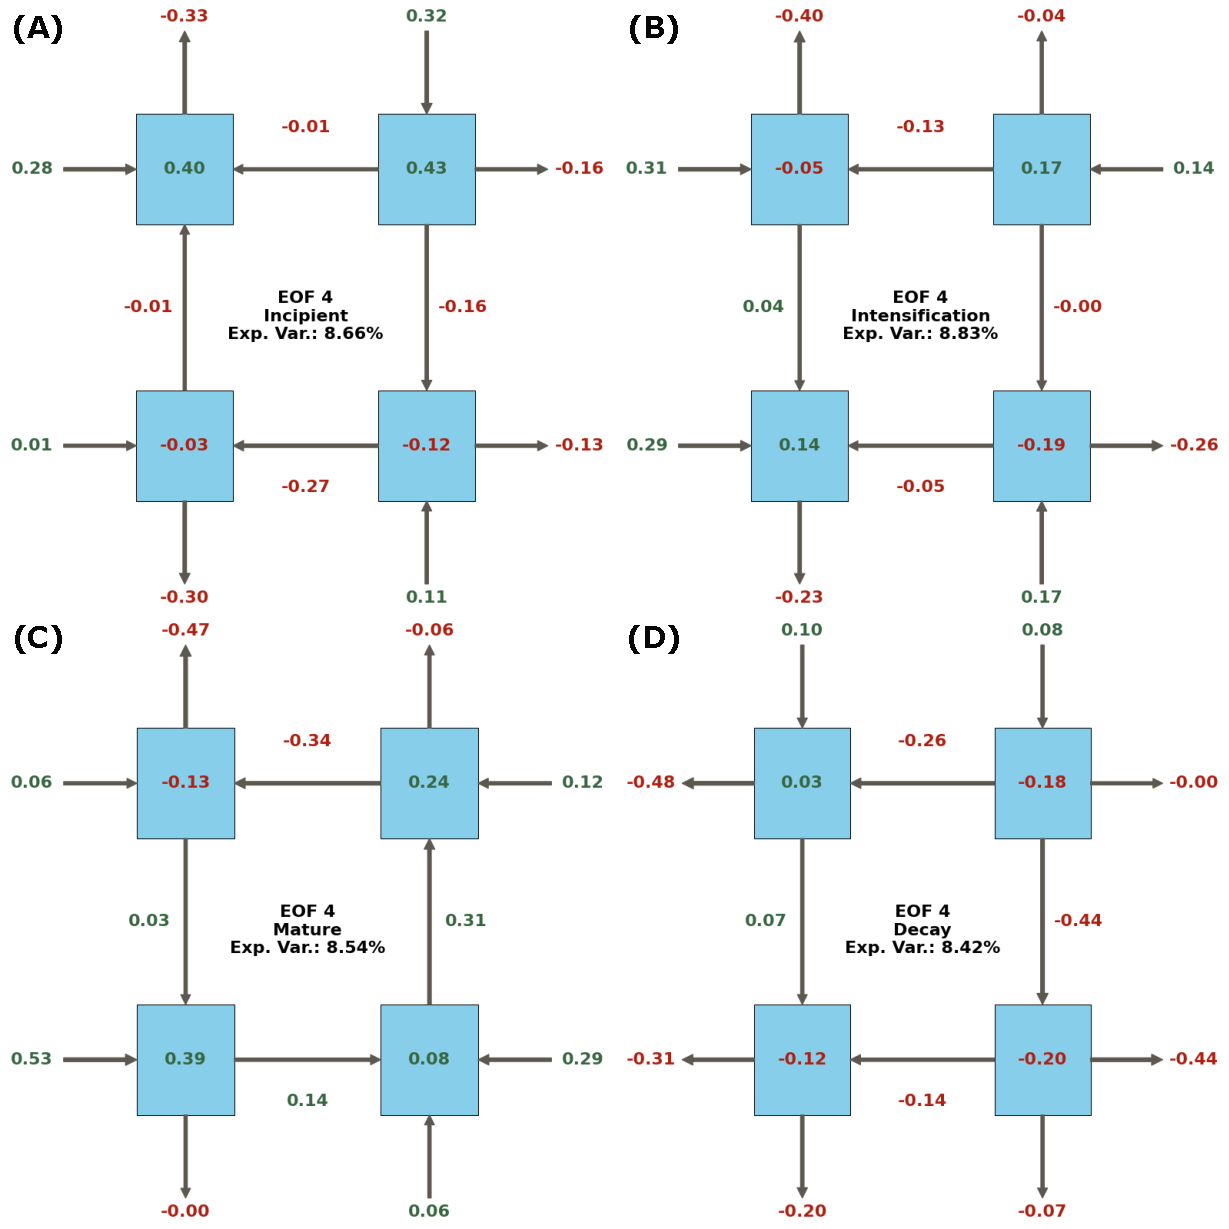
\includegraphics[width=\textwidth]{eof4_phases.pdf}
\caption{Lorenz Energy Cycle (LEC) terms for the fourth Empirical Orthogonal Function (EOF 4) across different life cycle phases: (A) incipient, (B) intensification, (C) mature, and (D) decay.}
\label{fig:eof4_phases}
\end{figure}

\subsection{Systems Statistics}

In this section, as the characteristics of the systems associated with each EOF are analyzed, the EOF signal becomes relevant, necessitating a distinction between systems related to positive EOF signals — EOF(+) — and negative EOF signals — EOF(-), respectively. EOF1 accounts for the largest number of cyclones among the first four EOFs for both EOF(+) and EOF(-). For EOF(+), it is followed by EOF2, EOF3, and EOF4, while for EOF(-), it is followed by EOF3, EOF2, and EOF4, respectively (Supplementary Figure S1a). The track densities for the cyclones associated with EOF(+) are presented in Figure \ref{fig:density_panel_q90}, while those for EOF(-) are shown in Figure \ref{fig:density_panel_q10}. For EOF1(+), the track density maximum extends from SE-BR and LA-PLATA toward the ARG region, highlighting the significant contribution of systems originating in the former regions compared to the latter, as also indicated in Figure \ref{fig:panel_2x2_eof_statistics}a. In contrast, for the remaining EOFs(+), the track density maximum is located near the ARG region, as most systems originate there. An exception is observed in EOF3(+), where the track density maximum extends northeastward due to the increased contribution of SE-BR systems to this EOF.


\begin{figure}[!htbp]
\centering

\includegraphics[width=\textwidth]{density_panel_q90.png}
\caption{Cyclone track density for the systems associated with EOFs(+): (A) EOF1, (B) EOF2, (C) EOF3, and (D) EOF4. The track density unit is cyclones per $10^{6}$ km$^{2}$ per month.}
\label{fig:density_panel_q90}
\end{figure}

\begin{figure}[!htbp]
\centering

\includegraphics[width=\textwidth]{density_panel_q10.png}
\caption{Cyclone track density for the systems associated to EOFs(-): (A) EOF1, (B) EOF2, (C) EOF3 and (D) EOF4. The track density unit is cyclone per $10^{6}$ $km^{2}$ per month.}
\label{fig:density_panel_q10}
\end{figure}

Meanwhile, EOFs(-) exhibit a more variable behavior. EOF1(-) displays two track density maxima: one near SE-BR and another near ARG, as fewer systems originate from LA-PLATA for this EOF (Figure \ref{fig:panel_2x2_eof_statistics}c). EOF2(-) is predominantly influenced by ARG systems, whereas EOF3(-) shows an increased contribution from LA-PLATA systems, with a primary track density maximum near ARG and a secondary maximum over the La Plata River mouth. Lastly, EOF4(-) presents a track density maximum between LA-PLATA and SE-BR, reflecting the increased relative contribution of systems from these regions to this EOF.

Despite these regional differences in track density maxima, all EOFs exhibit a common pattern of cyclone tracks extending southeastward across the South Atlantic. Some systems display exceptional mobility, reaching as far as $150^{\circ}$E. This behavior aligns with the typical lifecycle of cyclonic systems originating near the South American coast, where cyclones generally develop near the coastal region, mature as they propagate southeastward, and decay closer to the Antarctic region \citep{couto2024new}.

As shown in Figure \ref{fig:panel_2x2_eof_statistics}b, EOF1(+) and EOF4(+) systems predominantly originate during JJA, while EOF2(+) and EOF3(+) genesis events are more evenly distributed across the seasons. For EOFs(-), EOF1(-) systems occur mainly during DJF, whereas EOF4(-) systems are more frequent during DJF and MAM. In contrast, EOF2(-) and EOF3(-) systems are predominantly observed during JJA and SON (Figure~\ref{fig:panel_2x2_eof_statistics}d). The seasonal distribution of EOF2(+) and EOF3(+) systems aligns with the expected behavior, as ARG systems are well-distributed throughout the year \citep{gramcianinov2019properties,crespo2021potential}. However, for the remaining EOFs, the observed behavior suggests that seasonal variations are linked to changes in the systems' energetics.

\begin{figure}[!htbp]
\centering

\includegraphics[width=\textwidth]{panel_2x2_q90_vs_q10.png}
\caption{Genesis proportion and seasonal occurrences of EOFs. (A) Genesis proportion for EOF(+), (B) Seasonal occurrences for EOF(+), (C) Genesis proportion for EOF(-), and (D) Seasonal occurrences for EOF(-). The colors represent different genesis regions (ARG, LA-PLATA, SE-BR) in (A) and (C), while in (B) and (D), the colors correspond to seasonal distributions (DJF, MAM, JJA, SON).}
\label{fig:panel_2x2_eof_statistics}
\end{figure}

\subsection{Groups of Intense Systems}

While the previous sections examined the LEC for all cyclonic systems in the South Atlantic — analyzing both the mean behavior and its associated variability through EOF analysis — this section focuses on the energetic groups associated with the most intense cyclones in the dataset. The K-Means algorithm was applied to the first eight PCs of the selected cyclones, identifying five distinct LEC groups, as determined by the Elbow Method. Following the cluster identification analysis, the energetic characteristics of the systems were reconstructed, with the mean behavior for each group represented in Figure \ref{fig:LEC_clusters_std}.

\begin{figure}[!htbp]
\centering
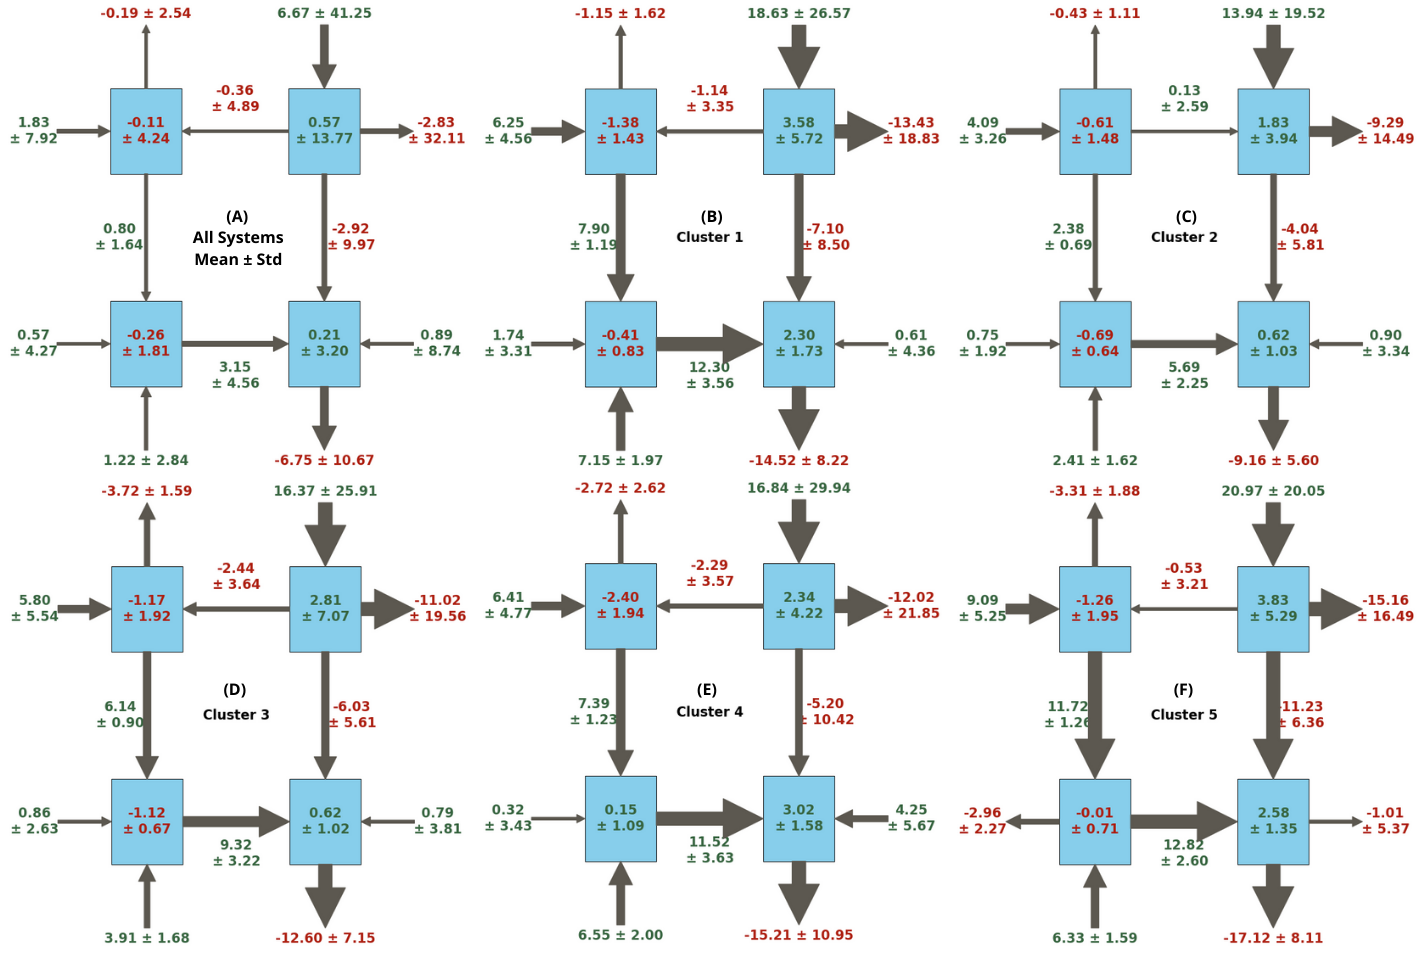
\includegraphics[width=\textwidth]{LEC_clusters_std.png}
\caption{(A) Mean values and standard deviations of the limited-area Lorenz Energy Cycle (LEC) terms for all analyzed systems. Panels (B–F) illustrate the reconstructed LEC for the five clusters identified among the most intense cyclones in the dataset, defined as systems with maximum central relative vorticity at 850 hPa exceeding the 99th percentile.}
\label{fig:LEC_clusters_std}
\end{figure}

Comparing the energy fluxes of the clusters with the mean behavior provides insight into the mechanisms that make these systems the most intense. Cluster 1 exhibits a three- to seven-fold increase in the moist baroclinic chain terms and a 2.5-fold increase in barotropic conversions, with both \( C_A \) and \( C_K \) contributing similarly for the \( K_E \) budget. Additionally, imports of \( K_E \) are below the average. Cluster 2 shows more modest increases, representing the cluster with the least enhanced energy fluxes. It experiences approximately a two-fold increase in both the moist baroclinic chain and barotropic conversions, while imports of \( K_E \) remain close to the mean values. Cluster 3 displays similar proportions to Cluster 2 for \( C_A \) and \( C_K \), though with slightly lower values. In contrast, \( C_E \) is one of the smallest among all clusters, second only to Cluster 2, primarily due to a relatively small \( G_E \). Additionally, Clusters 2 and 3 exhibit the lowest \( K_E \) budget values among all clusters. Cluster 4 features moist baroclinic chain values comparable to Cluster 1, albeit slightly lower. However, \( C_K \) is among the smallest of all clusters (second only to Cluster 2). This cluster stands out for its exceptionally high imports of \( K_E \), which are 4.7 times greater than the average, resulting in the highest \( K_E \) budget values among the clusters. Finally, Cluster 5 exhibits the highest values for baroclinic and barotropic conversion terms, with \( G_E \) values similar to those of Cluster 4. However, it is the only cluster displaying negative \( BK_E \) values, indicating net energy exports.

For all clusters, the residual term appears to be somewhat proportional to the \( K_E \) budget, though exceptions exist. Notably, this term is largest for Cluster 5, despite it having the second-highest \( K_E \) budget, whereas the highest \( K_E \) budget occurs in Cluster 4, which has the second-highest dissipation. This indicates that although most of the residual term's magnitude can be attributed to dissipative processes, subgrid processes and residual errors remain relevant factors.

Figure \ref{fig:density_panel} displays the track density for all clusters. For all clusters, the track density maxima extend from a region near the southeastern South American coast, between $30^\circ S$ and $50^\circ S$, propagating southeastward toward the Antarctic region. Cluster 1 systems exhibit a more concentrated track density, suggesting a preferential displacement path for these cyclones (Figure \ref{fig:density_panel}a). In contrast, Clusters 2 and 4 show track density maxima in two distinct regions: one over the LA-PLATA and SE-BR regions and another near Antarctica (Figure \ref{fig:density_panel}c and d). While the track density maxima near LA-PLATA and SE-BR are associated with the incipient and intensification phases of these systems, the maxima near Antarctica correspond to their decay phase \citep{couto2024new}. Cluster 3 presents a primary track density maximum extending from the LA-PLATA region, along with secondary maxima southeastward of it, located over the southeastern South Atlantic (SE-SAO), below South Africa, and near Antarctica (Figure \ref{fig:density_panel}c). Lastly, Cluster 5 exhibits a track density maximum between the ARG and LA-PLATA regions, with tracks predominantly extending eastward toward SE-SAO (Figure \ref{fig:density_panel}e). The SE-SAO region is associated with either cyclones undergoing a secondary life cycle \citep{couto2024new} or secondary cyclogenesis \citep{gramcianinov2019properties}.

\begin{figure}[!htbp]
\centering

\includegraphics[width=\textwidth]{density_panel.png}
\caption{Cyclone track density for the five clusters (A–E) identified among the most intense cyclones in the dataset. These systems are defined as those with maximum central relative vorticity at 850 hPa exceeding the 99th percentile.}
\label{fig:density_panel}
\end{figure}

Figure \ref{fig:cluster_analysis_panel} explores the mean characteristics of the cyclones associated with each cluster of intense systems. Among the five clusters, Cluster 2 contains the largest number of systems, followed by Clusters 3, 5, 1, and, finally, 4 (Figure~\ref{fig:cluster_analysis_panel}a). Notably, there is an inverse relationship between the number of systems in a cluster and their average maximum intensity, although significant intra-cluster variability is observed (Figure~\ref{fig:cluster_analysis_panel}b). As the \( K_E \) budget is positive during the incipient and intensification phases and negative during the mature and decay phases (Figure \ref{fig:panel_lec_mean_phases}), large values of \( K_E \) averaged over the entire life cycle indicate systems that acquire substantial kinetic energy during their intensification phase and, consequently, exhibit very intense cyclonic vorticity. This is exemplified by Cluster 4, which shows the highest \( K_E \) budget values while also presenting the highest mean maximum cyclonic vorticity values.

Most clusters are more frequent during JJA, followed by either SON or MAM (Figure \ref{fig:cluster_analysis_panel}c). The exception is Cluster 2, which occurs most frequently during SON and least frequently during JJA. This seasonality aligns with the expectated behavior, as LA-PLATA is the most frequent genesis region across all clusters (Figure \ref{fig:cluster_analysis_panel}d), consistent with the seasonal behavior of this region \citep{gramcianinov2019properties,crespo2021potential}. Furthermore, the prominence of LA-PLATA as the most frequent genesis region is also expected, as this region produces, on average, more intense systems compared to the other genesis regions \citep{gramcianinov2019properties}.


\begin{figure}[!htbp]
\centering

\includegraphics[width=\textwidth]{cluster_analysis_panel.png}
\caption{Characteristics of the five clusters (A–E) identified among the most intense cyclones in the dataset. (A) Number of cyclones per cluster, (B) maximum intensity (defined as maximum central relative vorticity at 850 hPa), (C) seasonal distribution of occurrences, and (D) genesis region count. In (C), colors represent different seasons (DJF, MAM, JJA, SON), while in (D), colors correspond to genesis regions (ARG, LA-PLATA, SE-BR).}
\label{fig:cluster_analysis_panel}
\end{figure}


\section{Discussion}\label{sec:discussion}

\subsection{Key Features}\label{sec:comparison}

The LEC diagrams (Figure \ref{fig:panel_lec_mean_phases}) indicate that the mean energetic behavior is preserved across the distinct life cycle phases. However, the high variability observed in Figure \ref{fig:combined_ridge} suggests that individual cyclones in the South Atlantic exhibit a wide range of behaviors. This section discusses the behavior inferred from the mean energy cycle and although emphasis is placed on the energy budget terms, it is important to note that this serves only as a starting point for understanding the energy sources of cyclones. These terms should not be analyzed in isolation; rather, the energy conversions and fluxes provide more meaningful indicators of the atmospheric dynamical processes occurring in the cyclone environment. In addition to the phase-specific diagrams (Figure \ref{fig:panel_lec_mean_phases}), a more intuitive schematic of the mean Lorenz Energy Cycle for all systems combined is presented in Figure \ref{fig:draw_LEC_total}. This diagram provides a simplified visualization of the mean energy exchanges, facilitating comparison across phases and identification of dominant conversion pathways.

\begin{figure}[!htbp]
\centering
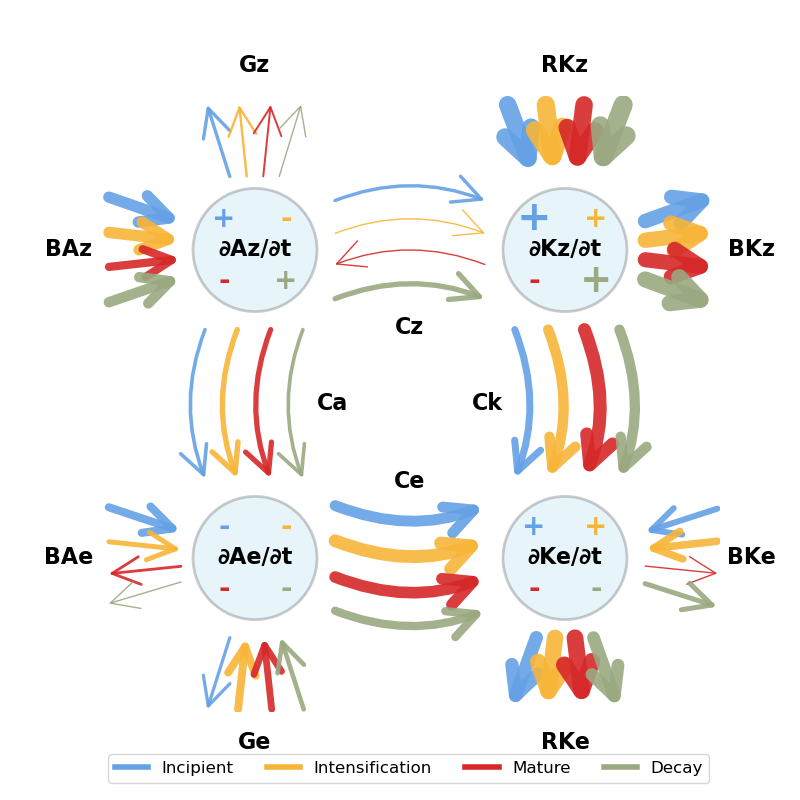
\includegraphics[width=\textwidth]{LEC_total_v6.png}
\caption{Schematic representation of the mean Lorenz Energy Cycle (LEC) for all analyzed cyclones in the South Atlantic, combining information from all life cycle phases. Arrows represent energy fluxes between reservoirs, with colors indicating the life cycle phases. The arrow thicknesses and symbol sizes for the balance terms ($\partial/\partial t$) are proportional to the absolute magnitude of each term, as presented in Figure \ref{fig:panel_lec_mean_phases}.}
\label{fig:draw_LEC_total}
\end{figure}

The $A_Z$ term initially increases, not due to a positive $G_Z$, but rather through a constant influx across the boundaries ($BA_Z > 0$). As baroclinic conversions increase during the intensification and mature phases, the $A_Z$ budget becomes negative, before returning to its initial trend during the decay phase. These results suggest that the initial and subsequent increases in $A_Z$ are not driven by diabatic heating at warmer latitudes coupled with diabatic cooling at colder latitudes. A similar temporal evolution for the $A_Z$ budget was found by \citet{dias2011energy} in their analysis of three cyclones along the South American coast. However, the use of relative vorticity at 850 hPa in this study allows for cyclone identification before the appearance of closed isobars at the surface \citep{sinclair1994objective,hoskins2002new}. In contrast, in \citet{dias2011energy}, the cyclone formation phase already presents a closed sea level pressure center, thus excluding the incipient phase from their analysis.

Regarding the $K_Z$ term, it shows an increasing trend across most phases of cyclone development, except during the mature phase. At this stage, barotropic conversions ($K_Z \rightarrow K_E$) are strongest, and $C_Z$ becomes negative, indicating descending motion at warmer latitudes and ascending motion at colder latitudes as the cold front reaches the equatorward side of the cyclone and the warm front reaches the poleward side. One prominent feature related to $K_Z$ is the large values of $BK_Z$ and, especially, $RK_Z$. The former shows a constant export of zonal kinetic energy, possibly associated with jet stream energy leaving the computational domain. The latter is difficult to interpret, as it includes terms related to boundary work ($B\Phi Z$), kinetic energy dissipation ($D_Z$), subgrid-to-grid scale energy transfer, and numerical errors accumulated during the computation of other terms. Although studies like \citet{dias2011energy} report values for $RK_Z$ comparable to those found here, they generally present such magnitudes only for specific development phases. These terms presented by works such as \citet{pezza2010environmental}, \citet{black2013universal}, and \citet{dias2013synoptic} show the same order of magnitude as the other energy fluxes.

The $A_E$ term consistently decreases across all phases, with minimal budget values during the incipient and intensification phases (one or two orders of magnitude smaller than the other terms). This is largely a result of the active, and highly efficient, baroclinic chain throughout the cyclone's life cycle. Energy is continuously supplied from the zonal available potential energy ($A_Z$) via the $C_A$ term, driven by meridional heat transport from frontal structures. Additionally, $A_E \rightarrow K_E$ conversions occur due to ascending air in the cyclone's warm sector and subsiding air in the cold sector. During the incipient and intensification phases, imports of $A_E$ keep this term only marginally negative. In the intensification phase, baroclinic conversions peak, and although imports decrease, the $G_E$ term becomes positive, driven by convective activity along the cyclone’s cold front \citep[e.g.][]{govekar2011three}. 

During the intensification phase, the cyclone's frontal structures are prominent, with low-level cloud formation dominating in the cold sector, leading to radiative cooling by cloud tops \citep{govekar2011three,voigt2023tug}. Simultaneously, radiative heating occurs in the warm sector due to long-wave absorption from mid- to high-level clouds \citep{lau1997comparing,keshtgar2023cloud}. These combined effects enhance $G_E$. Furthermore, during the intensification period the precipitation is most intense \citep{mcerlich2023assessment}, releasing latent heat. In the mature phase, as both meridional heat transport and vertical motion in the cyclone's cold and warm sectors weaken, the reversal of $BA_E$ to signal exports of this form of energy, combined with reduced convective activity, leads to a sharp decrease in $A_E$. By the decay phase, the baroclinic chain further weakens, convective activity declines, and the cyclone's frontal structures become diffuse and lose organization, leading to smaller values of $G_E$ due to diminished cloud radiative effects. As boundary transport becomes more neutral, the $A_E$ budget returns to levels similar to those in the incipient and intensification phases.

Meanwhile, $K_E$ exhibits an increasing trend during the incipient and intensification phases, followed by a decrease during the mature and decay phases. In the earlier phases, energy supplied by the baroclinic chain, barotropic conversion, and imports offsets the losses due to $RK_E$. However, in the mature stage, despite an increase in barotropic conversion, the reversal of the boundary term, along with a reduction in the baroclinic chain and an increase in $RK_E$, results in a negative $K_E$ budget. During the decay phase, even though $RK_E$ returns to its initial values, the decreasing energy supply to $K_E$ and increasing exports lead to the term's budget reaching its minimum value, signaling the cyclone's dissipation. Although the $RK_E$ term also aggregates numerical errors and includes the $B\Phi E$ term, similar to $RK_Z$, the results suggest that much of this term's signal is related to energy dissipation, consistent with \citet{smith1980energetics}.

Both $B\Phi Z$ and $B\Phi E$ were directly computed to allow comparison with the residual terms, resulting in excessively large values (Table \ref{tab:lec_stats} and Figure \ref{fig:combined_ridge}d). As noted by \citet{brennan1980zonal}, these terms represent the work done by zonal and meridional wind components against atmospheric pressure at the boundaries of the computational domain. However, small errors in the geopotential height field can escalate into significant deviations in these terms, potentially biasing the results. Although ERA5 dataset post-processing includes quality control, small deviations in the geopotential field may still exist in the dataset. Since the LECTK program does not include a preprocessing quality control, any such deviations were likely carried into the analysis. Future work should further investigate the physical mechanisms underlying the $B\Phi Z$ and $B\Phi E$ terms and explore potential causes for the large values observed. Direct comparisons with other studies are difficult, as values for these terms are rarely reported.

\subsection{Cyclone Groups}

However, substantial variability exists within the dataset, as revealed by the EOF analysis. Most of this variability is captured by EOF1(+) and EOF1(-), each associated with nearly 20\% of the systems in the dataset. While EOF1(+) is related to relatively stronger systems, EOF1(-) corresponds to relatively weaker systems (Supplementary Figure S1). This indicates that a significant portion of the analyzed systems exhibit a bi-modal behavior, with "day-to-day" cyclones being either relatively weak or intense, as a result from their energy cycle. Traditional cyclone climatologies over the South Atlantic tend to group all cyclones together \citep[e.g.,]{sinclair1994objective,hoskins2005new,reboita2010south,gramcianinov2019properties}. In contrast, the results presented here suggest that these systems exhibit distinct behaviors and may therefore be categorized into separate groups.

The intensity differences between these systems are also reflected in their LEC patterns and associated characteristics. A schematic representation of the Lorenz Energy Cycle for each of the four leading EOFs is presented in Figure \ref{fig:EOFs_panel}, allowing a direct comparison of their dominant energetic pathways. EOF1(+) is largely linked to an enhancement of mean energy fluxes across all life cycle stages (Figure \ref{fig:draw_LEC_total}), whereas EOF1(-) exhibits the opposite behavior. Additionally, this intensity distinction impacts the mobility of these systems. EOF1(+) systems are significantly more mobile, with their track densities closely following the South Atlantic storm tracks \citep{hoskins2005new,gramcianinov2019properties}. In contrast, EOF1(-) systems are more concentrated near the South American coast (Figure \ref{fig:density_panel_q10}a), mostly related to ARG and SE-BR systems (Figure \ref{fig:panel_2x2_eof_statistics}d), exhibiting lower mobility and reduced translational speed (Supplementary Figure S1).

\begin{figure}[!htbp]
\centering
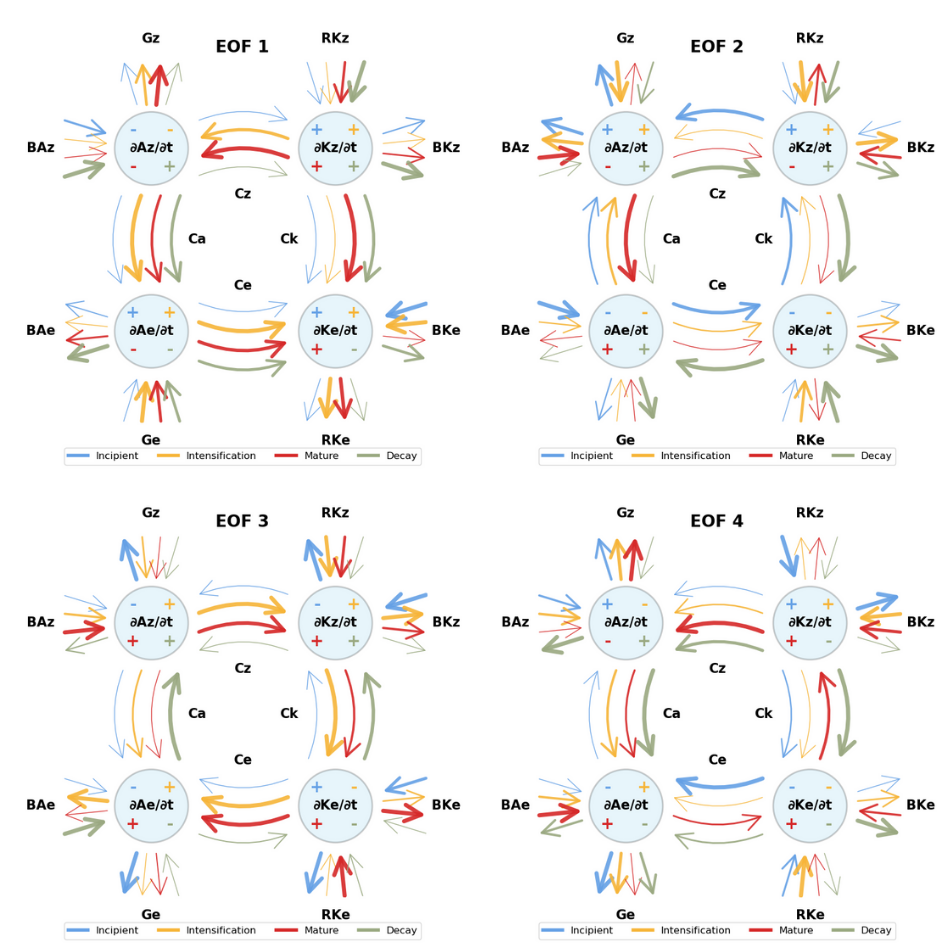
\includegraphics[width=\textwidth]{EOFs_panel.png}
\caption{Schematic representation of the mean Lorenz Energy Cycle (LEC) for cyclones associated with the four four leading positive Empirical Orthogonal Functions (EOF1(+) to EOF4(+)). Arrows represent energy fluxes between reservoirs, with colors indicating life cycle phases. The thickness of each arrow and the size of the balance terms ($\partial/\partial t$) symbols are proportional to the absolute magnitude of each term.}
\label{fig:EOFs_panel}
\end{figure}

EOF2, EOF3, and EOF4 represent less common cyclone types. EOF2(+), EOF3(-), and EOF4(-) are associated with relatively strong systems, whereas their counterparts (EOF2(-), EOF3(+), and EOF4(+)) correspond to relatively weak systems (Supplementary Figure S1).  EOF2(+) exhibits a distinctive behavior in that neither baroclinic nor barotropic conversions, nor the imports of \( K_E \), are enhanced during the incipient and intensification phases. In contrast, EOF3(-) shows an enhancement of barotropic conversions during the incipient phase, as well as an intensification of the \( G_E \rightarrow A_E \rightarrow K_E \) chain during both the incipient and intensification phases. Similarly, EOF4(-) features an enhancement of the \( G_E \rightarrow A_E \rightarrow K_E \) chain during its intensification phase, while during the incipient phase, the moist baroclinic chain is significantly strengthened. Furthermore, when we look at each PC contribution for each intense system (above the q99 maximum central vorticity threshold), there is an overall predominance of EOF1(+) and EOF3(–) (Supplementary Figure S2). These results indicate that, although the cyclonic systems in the South Atlantic region share a predominant energy cycle, the intrinsic variability — expressed through deviations in the energy pathways — reveals that these systems possess distinct characteristics. This variability is further reflected in the different groups exhibiting distinct preferred genesis regions and seasonality (Figure \ref{fig:panel_2x2_eof_statistics}).

For the most intense systems, the observed seasonality (mostly during JJA) and preferred genesis region (LA-PLATA) are expected, as previous studies have identified this region as generating more intense systems \citep{reboita2010south,gramcianinov2019properties} and with higher frequency during JJA \citep{crespo2021potential}. Here, we also show that, despite barotropic conversions playing an important role in their development, these systems are primarily attributed to moist baroclinic instability (Figure~\ref{fig:LEC_clusters_std}). During austral winter, these systems develop in a strongly baroclinic environment, supported by a robust upper-level jet \citep{gramcianinov2019properties,crespo2021potential}.

Cluster 2 is an exception to this pattern, with more frequent cyclogenesis occurring during the warmer months. These systems exhibit the highest \( C_K/C_A \) ratio. Additionally, there is an increased proportion of genesis over SE-BR for these systems compared to the other clusters. The weaker baroclinicity in this region and season has been previously reported \citep{gramcianinov2019properties,crespo2021potential}, alongside the enhancement of barotropic conversions \citet{dias2011energy}. Overall, these results not only reinforce the argument for distinct groups among cyclones in the South Atlantic but also highlight substantial differences between weaker/moderate systems and the more intense ones. Furthermore, even within the intense cyclone systems, there is significant heterogeneity in their energy cycles and behavior.

\subsection{Mechanisms of Energy Transfer}

Thorough the present study, an interesting although unsettling result became evident, that barotropic conversions (denoted by the $C_K$ term) are one important feature for cyclonic systems development in South America region. These results are unexpected as traditionally extratropical cyclones - the vast majority of systems in the South Atlantic \citep{marrafon2022classificaccao} - are mainly associated with baroclinic instability process \citep{bjerknes1922life,charney1964growth,hoskins1990existence}. Over the life cycle of the cyclones, the moist baroclinic chain serves as the primary energy source for \( K_E \), with its contribution peaking during the intensification phase, while barotropic conversions peak at the mature stage (Figure \ref{fig:panel_lec_mean_phases}). Furthermore, the magnitude of \( C_K \) is nearly three times that of the \( C_A \) term, suggesting a more substantial energy supply to eddy development from the zonal flow kinetic energy compared to the meridional temperature gradients.

Although studies investigating the LEC of cyclonic systems date back to the last century, such studies remain scarce, particularly for the South Atlantic region, which limits the direct comparison of results. For tropical systems, the limited case studies available highlight the importance of the \( G_E \rightarrow A_E \rightarrow K_E \) chain and barotropic conversions \citep{brennan1980zonal,veiga2008analysis}. For subtropical systems, the energy pathways supplying \( K_E \) exhibit variable behavior throughout their lifecycle and both baroclinic and barotropic conversions appear to be significant mechanisms for their development \citep{michaelides1987limited,dias2013synoptic,pezza2014large,cavicchia2018energetics}. Finally, for extratropical systems, particularly during their development phase, cyclones seem to display a wide range of behaviors. These behaviors include systems dominated by pure baroclinic conversions \citep{dias2011energy,black2013universal}, systems dominated by barotropic conversions \citep{michaelides1992spatial,dias2011energy}, that may also be accompanied by imports of \( K_E \) \citep{wahab2002mechanism}, or systems involving a combination of both conversions \citep{bulic2006limited,pezza2010environmental}.

Thus, although the predominance of barotropic conversions (and therefore barotropic instability) over the baroclinic chain (baroclinic instability) in the energy cycle of extratropical cyclones —particularly in the South Atlantic region — is not a pioneering result, this study presents the first analysis of such a large number of systems, providing a consolidated view of this behavior. It is also important to emphasize that, while previous studies investigated the LEC using an Eulerian framework, this study employed a semi-Lagrangian framework. This approach has the advantage of isolating the energetics strictly related to the target system. However, the extent to which this methodology differs from the Eulerian framework in representing the magnitude and direction of energy fluxes has not been extensively assessed, apart from one study by \citet{michaelides1999quasi}.

Moreover, it remains unclear how much of the presented results can be generalized to other regions. For instance, given that Southern Hemisphere jets are more intense and exhibit a stronger meridional gradient of the \( u \)-wind component \citep[e.g.,][]{swart2019canadian,jain2023monsoon,savita2023assessment}, it is expected that barotropic conversions in the South Atlantic might be more intense than those observed in the North Atlantic. However, this hypothesis requires further investigation.


\section{Summary and Conclusions}\label{sec:conclusion}

In this study, we examined the Lorenz Energy Cycle (LEC) for 7,531 cyclonic systems originating in the Southwestern Atlantic, presenting what is, to the best of our knowledge, the first comprehensive climatology of cyclones' energy cycles in this region. A notable exception is the work by \citet{black2013universal}, which focused solely on explosive cyclones and used large fixed domains, contrasting with the semi-Lagrangian approach adopted in this study. While studies such as \citet{smith1980energetics} provide valuable reviews of the energetics of extratropical cyclones, focusing on broad averages and generalized mechanisms, and case studies have explored the dynamics of specific systems \citep[e.g.]{pezza2014large,dias2011energy,cavicchia2018energetics}, our study adopts a climatological approach. Specifically, we track the energy cycles of individual cyclones across distinct life cycle phases, offering a more detailed investigation of the unique physical mechanisms that drive energy conversions in this region. Furthermore, the use of the Cyclophaser program to dissect the life cycles of cyclones has enabled a novel investigation of the energy cycle across different developmental stages, providing deeper insights into the variability and dynamism of these systems.


The results presented here demonstrate that, for most cyclonic systems in the South Atlantic, a clear pattern of energy flow is evident. This pattern is characterized by both barotropic and baroclinic conversions providing energy for eddy development and is preserved throughout the cyclone life cycle phases, despite variations in magnitude. Barotropic conversions tend to be 2 to 3 times larger in magnitude than baroclinic conversions, with the former peaking during the mature phase and the latter during the intensification phase. The generation of eddy potential energy and the imports of eddy kinetic energy play secondary roles. The former peaks during the intensification phase and remains positive through the mature and decay phases, while the latter occurs primarily during the incipient (cyclogenesis) and intensification phases.

Despite the high variability among the systems, the EOF analysis indicates that, in most cases, the main behavior is preserved. This variability is instead expressed as a strengthening and/or weakening of specific energy pathways, indicating that cyclonic development in the South Atlantic region can be attributed to distinct dynamical processes, as supported by the literature. Consequently, it is possible to hypothesize that these systems can be grouped into distinct types based on their characteristics and energy cycles. This heterogeneity is also evident among the most intense systems. For these systems, distinct groups exhibit varying relative contributions of energy from barotropic and baroclinic chains, as well as differences in eddy generation of APE and imports of eddy kinetic energy. Although most of these intense systems originate in the LA-PLATA region, the variability in the relative proportions of genesis regions among the different clusters is reflected in their energy cycles and mean characteristics.

The goal of this study was to investigate the energy cycle of cyclones in the South Atlantic region using a semi-Lagrangian approach. As a pioneering study of this kind, several questions have emerged throughout its development. For instance, previous studies for this region have assessed the distinct synoptic and dynamical conditions related to cyclogenesis in the three primary genesis regions \citep{gramcianinov2019properties,crespo2021potential}. A distinction in the energy cycles among these genesis regions would therefore be valuable. Additionally, given the prominence of barotropic conversions as an energy source for cyclone development, the question arises as to whether barotropic instability is truly occurring near the cyclone center. \citet{souza2024thesis} proposed a framework for classifying cyclones into distinct groups based on their energy cycles. In an upcoming study, this method will be applied to address these questions and further investigate these topics.


\backmatter

\bmhead{Supplementary information}

If your article has accompanying supplementary file/s please state so here. 

Authors reporting data from electrophoretic gels and blots should supply the full unprocessed scans for key as part of their Supplementary information. This may be requested by the editorial team/s if it is missing.

Please refer to Journal-level guidance for any specific requirements.

%TC:ignore
\section*{Declarations}

\subsection*{Funding}

This study was partly financed by the Coordenação de Aperfeiçoamento de Pessoal de Nível Superior – Brasil (CAPES) under Finance Code 001.

\subsection*{Competing interests}

The authors have no relevant financial or non-financial interests to disclose.

\subsection*{Data Availability}

The cyclone tracks used in this study were obtained from the \textit{Atlantic Extratropical Cyclone Tracks Database}, available at \url{https://doi.org/10.17632/kwcvfr52hp.4}. All datasets, including the computed Lorenz Energy Cycle results for each cyclone, along with the scripts used to generate the figures and analyses presented in this study, are publicly available at the following GitHub repository: \url{https://github.com/daniloceano/energetic_patterns_cyclones_south_atlantic}. The source code of the \texttt{Cyclophaser} package, used for detecting cyclone life cycle phases, is available on PyPI at \url{https://pypi.org/project/cyclophaser/}. The \texttt{LorenzCycleToolkit} package, used for computing the Lorenz Energy Cycle components, is also available on PyPI at \url{https://pypi.org/project/LorenzCycleToolkit/}.

\subsection*{Author contributions}

Conceptualization: Danilo Couto de Souza, Pedro Leite da Silva Dias, Ricardo de Camargo, Carolina Barnez Gramcianinov; Methodology: Danilo Couto de Souza, Pedro Leite da Silva Dias, Ricardo de Camarg; Formal analysis and investigation: Danilo Couto de Souza, Pedro Leite da Silva Dias; Writing - original draft preparation: Danilo Couto de Souza; Writing - review and editing: Danilo Couto de Souza, Pedro Leite da Silva Dias, Ricardo de Camargo, Carolina Barnez Gramcianinov; Funding acquisition: Pedro Leite da Silva Dias, Ricardo de Camargo; Resources: Pedro Leite da Silva Dias, Ricardo de Camargo; Supervision: Pedro Leite da Silva Dias, Ricardo de Camargo.

\bibliography{sn-bibliography}% common bib file
%% if required, the content of .bbl file can be included here once bbl is generated
%%\input sn-article.bbl


\end{document}
